% Created 2023-03-21 Вт 19:30
% Intended LaTeX compiler: pdflatex
\documentclass[PI, VKR]{HSEUniversity}
                \Year{\the\year{}}
                                \supervisor{к.т.н.}{доцент кафедры информационных технологий в бизнесе НИУ ВШЭ-Пермь}{А. В. Бузмаков}
\Abstract{В данной работе проведен анализ этичности разных компаний.

В первой главе находится описание используемых алгоримов.

Во второй главе представлено проектирование системы.

В третьей главе представлена реализация системы.

В четвертой главе представлено тестирование работы системы.

Количество страниц -- \pageref*{pg:end}, количество иллюстраций -- \TotalValue{totalfigures}, количетсво таблиц -- \TotalValue{totaltables}.
}
\usepackage{amsmath}
\author{Соломатин Роман Игоревич}
\date{\today}
\title{Разработка сайта для автоматического сбора, анализа и визуализации информации по этичности компаний}
\hypersetup{
 pdfauthor={Соломатин Роман Игоревич},
 pdftitle={Разработка сайта для автоматического сбора, анализа и визуализации информации по этичности компаний},
 pdfkeywords={},
 pdfsubject={},
 pdfcreator={Emacs 28.2 (Org mode 9.6.1)},
 pdflang={Russian}}
\usepackage{biblatex}
\addbibresource{~/Desktop/notes/org/bibliography.bib}
\begin{document}

\maketitle

\chapter*{Введение}
\label{sec:org28365d6}
Этика компаний – это разделяемые всеми сотрудниками организации правила и нормы, ценности и убеждения, манера общения и другие факторы, которые регламентируют поведение и взаимодействии членов компании. Существует 3 уровня этики компаний\autocite{smirnova_biznesetika_2021}:
\begin{enumerate}
\item мировой -- отвечает за увеличение общественного благосостояния, обеспечение рабочих мест, научно-технические инновации и модернизацию производственных процессов и т. д.
\item макроуровень -- отвечает за принципы рыночной конкуренции, информационной прозрачность и равнодоступности для всех участников рынка и т. д.
\item микроуровне -- отвечает за доверие и отсутствие дискриминации в отношениях между контрагентами, между сотрудниками и менеджерами, морально-нравственный климат в организации и т. д.
\end{enumerate}
В данной работе будет рассматриваться этика на микроуровне.

Этичность компаний уже давно вызывает озабоченность, особенно их поведение в спорных ситуациях и предоставление услуг, ориентированных на клиента. В последние годы все большее внимание уделяется оценке этичности компаний\autocites{mure_esg_2021}[][]{semenko_korporativnaya_2022}[][]{kudryavceva_korporativnosocialnaya_2016}, особенно в банковском секторе и через призму экологических, социальных и управленческих факторов (ESG). Необходимость в таких оценках становится все более острой по мере того, как общество продолжает бороться с последствиями неправомерных действий корпораций и более широким воздействием корпоративной деятельности на общество и окружающую среду.

В настоящее время существует несколько сервисов, которые призваны оценивать этику компании на основании финансовых показателей\footnote{\url{https://kontur.ru/expert}, \url{https://www.esphere.ru/products/spk/financial}} и судебных дел\footnote{\url{https://proverki.gov.ru/portal/public-search}}. Это привело к ситуации, когда отдельные лица должны проводить свои собственные исследования, чтобы определить насколько этична компания. Это часто включает в себя просмотр отзывов с различных веб-сайтов, что может занять много времени и не всегда может дать исчерпывающую или точную картину, так как не включает в себя качество обслуживания.

Для решения этой проблемы реализована система, которая собирает и анализирует отзывы потребителей с различных веб-сайтов, чтобы дать более полную и точную оценку этической практики компании. Затем собранные данные анализируются с помощью различных методов, таких как обработка естественного языка и машинного обучения, для выявления закономерностей и тенденций, связанных с этической практикой компании. Полученный анализ может быть использован для разработки более надежной и достоверной системы оценки этичности компаний.

Объект исследования – взаимодействие компаний с клиентами.

Предмет исследования – программные средства для оценки этичности на основе взаимодействия компаний с клиентами.

Цель работы – создание системы для оценки этичности компаний.

Исходя из поставленной цели, необходимо:

\begin{enumerate}
\item Провести анализ предметной области и требований
\item Реализовать систему
\item Провести тестирование системы
\end{enumerate}

Этап анализа должен:
\begin{enumerate}
\item Анализ предметной области
\item Анализ требований к системе
\item Анализ существующих алгоритмов
\end{enumerate}

Этап проектирования должен включать:
\begin{enumerate}
\item Проектирование серверной части
\item Проектирование модели для определения этичности
\item Проектирование клиентской части приложения
\end{enumerate}

Этап реализации должен включать:
\begin{enumerate}
\item Описание сбора данных
\item Реализации модели
\item Реализации серверной части
\item Реализации клиентской части
\end{enumerate}

Этап тестирования должен включать:
\begin{enumerate}
\item Тестирование модели
\item Тестирование серверной части
\item Тестирование клиентской части
\end{enumerate}

В ходе выполнения анализа, проектирования и реализации приложения используется объектно-ориентированный подход. Результаты анализа и решения задач проектирования формализуются с помощью диаграмм \texttt{UML}. При разработке базы данных используется реляционная СУБД \texttt{PostgreSQL}, а серверная часть приложения реализуется на языке python с помощью фреймворка \texttt{FastApi}, а алгоритмы анализы текста будут использовать методы машинного обучения.
\chapter{Анализ предметной области}
\label{sec:org85db885}
В данной главе представлен аналитический обзор оценок этичности компаний и алгоритмов машинного обучения, а также обзор существующих программных решений для поставленной проблемы.

Анализ предметной области следует разделить на следующие пункты:
\begin{enumerate}
\item анализ процесса определения этичности компаний сейчас позволяет понять, как этот процесс сейчас происходит и как его лучше всего автоматизировать;
\item анализ оценок этичности компаний для того, чтобы в дальнейшем определить этичность компаний;
\item анализ существующих решений выполняется с целью выделения их сильных и слабых сторон по отношению к решаемой проблеме и обоснования необходимости разработки нового средства, подходящего под регламент задач;
\item анализ алгоритмов позволяет понять с помощью каких алгоритмов можно найти полезную информацию в текстах;
\item анализ требований к системе позволит выделить функциональные и не функциональные требования.
\end{enumerate}
\section{Анализ определения этичности компании}
\label{sec:org085e00d}
Сейчас процесс поиска этичной компании выгладит следующим образом: сначала ищутся компании, которые предоставляют желаемые услуги. Далее они изучаются, чтобы определить их этичность. Этот процесс включает в себя:
\begin{enumerate}
\item просмотр отчетности компании
\item анализ ее финансовой деятельности
\item изучение информации о социальной ответственности
\end{enumerate}

Для этого они обращаются к различным источникам информации, таким как веб-сайты компаний, рейтинговые агентства, исследовательские организации и другие источники. Потом, изучаются социальные сети компании или отзывы пользователей на разных сайтах, форумах и социальных сетях, чтобы получить дополнительную информацию и оценить общее мнение о компании. После изучения каждой компании люди выбирают ту, которую они считают наиболее этичной и социально ответственной. Блок-схема данного поиска рис. \ref{fig:as_is}. Важным фактором для определения этичности компании может быть ее социальная ответственность, устойчивость бизнеса и соблюдение норм и стандартов в области финансовой деятельности.

В целом, процесс поиска компаний и определения их этичности может быть длительным и требует серьезного подхода. Люди могут использовать различные источники информации, чтобы сделать осознанный выбор и инвестировать свои деньги в компанию, которая соответствует их ожиданиям и требованиям.
\begin{figure}[h]
\centering
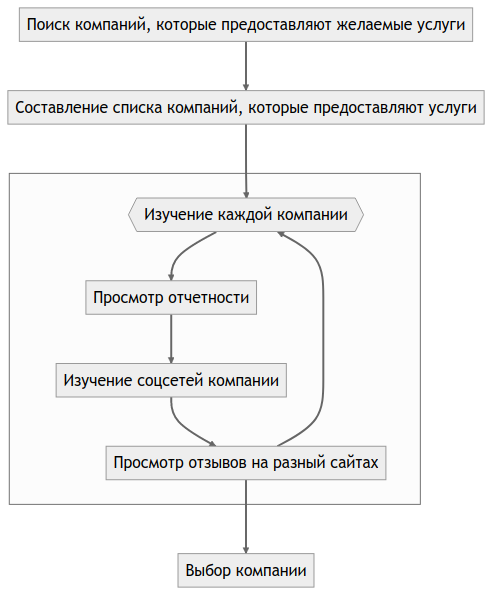
\includegraphics[width=0.6\textwidth]{img/mermaid/as_is.png}
\caption{\label{fig:as_is}Диаграмма того, как сейчас происходит поиск компании}
\end{figure}

\section{Анализ оценок этичности компаний}
\label{sec:orgc4b2b0f}
Оценка этики компании -- это не одноразовый процесс, а скорее непрерывная попытка понять и оценить действия, политику и практику компании с течением времени. Это включает в себя рассмотрение соблюдения компанией отраслевых этических стандартов и передовой практики, а также мониторинг любых изменений в этической позиции компании с течением времени. Кроме того, участие в диалоге с компанией и консультации с организациями, специализирующимися на оценке корпоративной ответственности могут дать ценную информацию об этических практиках компании.

Компаниям важно оставаться этичными, так как на долгосрочной перспективе это приносит большую прибыль и улучшает показатели бизнеса, чем неэтичный способ ведение бизнеса\autocites{climent_ethical_2018}[][]{mure_esg_2021}. Насколько этична компания можно рассматривать с двух сторон, самой компании и их клиентов. Со стороны компаний можно выделить факторы, которые можно получить из их отчетности:
\begin{itemize}
\item количество капитала, чтобы они не могли обанкротиться;
\item какое влияние они вносят на окружающую среду;
\item куда идут инвестиции\autocite{harvey_ethical_1995}.
\end{itemize}
Для пользователей одними из ключевых факторов можно выделить:
\begin{itemize}
\item качество пользовательского сервиса\autocite{brunk_exploring_2010}, как правило пользователи оставляют отзывы на сайтах по 5-ти бальной шкале;
\item насколько навязчивые услуги компании\autocite{mitchell_bank_1992}, как правило пользователи оставляют отзывы на сайтах по 5-ти бальной шкале.
\end{itemize}

В данной работе этичность компаний будет определяться по отзывам клиентов, которые освещают проблемы качества услуг и качество сервиса, и на основе отчетности компаний, что позволит полностью осветить проблему. Для анализа текстов будут использоваться алгоритмы машинного обучения.
\section{Анализ существующих решений}
\label{sec:org93af824}
Существует несколько индексов, предназначенных для измерения этичности -- индекс Доу Джонса (DJSI)\autocite{lopez_sustainable_2007} и FTSE4GOOD\autocite{collison_financial_2008}.

DJSI оценивает показатели устойчивости компаний различных секторов на основе экономических, экологических и социальных критериев. Компании отбираются на основе их показателей по сравнению с аналогичными компаниями в том же секторе. Процесс оценки включает в себя тщательную оценку компаний по различным критериям, включая корпоративное управление, экологический менеджмент, трудовую практику, права человека и социальные вопросы.

Аналогичным образом, индекс FTSE4GOOD предназначен для оценки деятельности компаний, которые демонстрируют эффективную практику экологического, социального и управленческого менеджмента (ESG). Компании отбираются на основе их практики ESG и оцениваются по различным критериям, включая изменение климата, права человека и корпоративное управление.

Индексы DJSI и FTSE4GOOD разработаны для того, чтобы помочь инвесторам определить компании, которые привержены этической практике. Эти индексы предоставляют инвесторам стандартизированный способ сравнения компаний на основе их показателей. Это помогает инвесторам принимать более обоснованные инвестиционные решения и побуждает компании внедрять устойчивую практику для привлечения инвестиций.

Для российских компаний нет аналогичных индексов. Сейчас данные об этичности компаний можно получить из агрегаторов отзывов и отчётности. Агрегаторы позволяют собрать информацию о клиентском обслуживании, а отчетность компаний о положении дел в целом. Но сейчас не существует способов, как можно оценить все вместе.
\section{Алгоритмы для анализа текста}
\label{sec:org9a41605}
Алгоритмы машинного обучения для анализа текста получили широкое распространение для извлечения информации из неструктурированных данных с помощью больших помеченных наборов данных. Среди различных используемых методов несколько алгоритмов оказались особенно эффективными в этой области. К ним относятся мешок слов\autocite{harris_distributional_1954}, TF-IDF\autocite{jones_karen_sparck_statistical_1972}, Word2Vec\autocite{mikolov_distributed_2013}, ELMO\autocite{peters_deep_2018}, GPT\autocite{radford_language_2019} и BERT\autocite{devlin_bert_2019}. Каждый из этих алгоритмов обладает уникальными характеристиками, которые делают их хорошо подходящими для определенных приложений.

Модель {}<<Мешок слов>>{} представляет текстовые данные путем присвоения уникального номера каждому слову в документе. Этот метод прост в реализации, но не учитывает порядок слов в предложении. С другой стороны, модель TF-IDF представляет текстовые данные, учитывая как частоту слова в документе (TF), так и его редкость во всех документах корпуса (IDF). Этот подход может быть использован для определения важности слова в данном документе и обычно используется в задачах поиска информации и обработки естественного языка, но он не понимает контекста слов.

Word2Vec использует векторное представление слов, что позволяет алгоритму улавливать значение слов в сходных контекстах. Это позволяет более точно и изощренно представлять взаимосвязи между словами, что приводит к повышению производительности в таких задачах, как классификация текста и анализ настроений.

ELMO, GPT и BERT, с другой стороны, основаны на архитектуре трансформеров, в которой каждое предложение представлено вектором чисел, обычно известным как вложение. Такое представление позволяет получить более полное и целостное понимание текста, поскольку оно учитывает контекст всего предложения или текста.

Из этих алгоритмов BERT считается наиболее продвинутым и мощным, поскольку он способен учитывать контекст всего предложения или текста, в то время как GPT и ELMO рассматривают только односторонний контекст. Это позволяет BERT достигать самых современных результатов в широком спектре задач анализа естественного языка.

Таблица результата сравнения моделей \ref{tbl:model_compare}.

\begin{table}[h!]
\caption{\label{tbl:model_compare}Сравнение моделей}
\centering
\begin{tabular}{|c|c|c|}
\hline
Модель & Вектор слов & Контекст\\[0pt]
\hline
Мешок слов & зависит от количества слов & нет\\[0pt]
\hline
TF-IDF & зависит от количества слов & очень слабо\\[0pt]
\hline
Word2Vec & не зависит от количества слов & слабо\\[0pt]
\hline
ELMO & не зависит от количества слов & однонаправленный\\[0pt]
\hline
GPT & не зависит от количества слов & однонаправленный\\[0pt]
\hline
BERT & не зависит от количества слов & двунаправленный\\[0pt]
\hline
\end{tabular}
\end{table}

\subsection{BERT}
\label{sec:orgadb9987}
BERT \autocite{devlin_bert_2019} (Bidirectional Encoder Representations from Transformers) -- это нейросетевая языковая модель, которая относится к классу трансформеров. Она состоит из 12 «базовых блоков» (слоев), а на каждом слое 768 параметров.

На вход модели подается предложение или пара предложений. Затем разделяется на отдельные слова (токены). Потом в начало последовательности токенов вставляется специальный токен \texttt{[CLS]}, обозначающий начало предложения или начало последовательности предложений. Пары предложений группируются в одну последовательность и разделяются с помощью специального токена \texttt{[SEP]}, затем к каждому токену добавляется эмбеддинг, показывающий к какому предложению относится токен. Потом все токены превращаются в эмбеддинги \ref{fig:inputemebeddings} по механизму описаному в работе \autocite{vaswani_attention_2017}.

\begin{figure}[h]
\centering
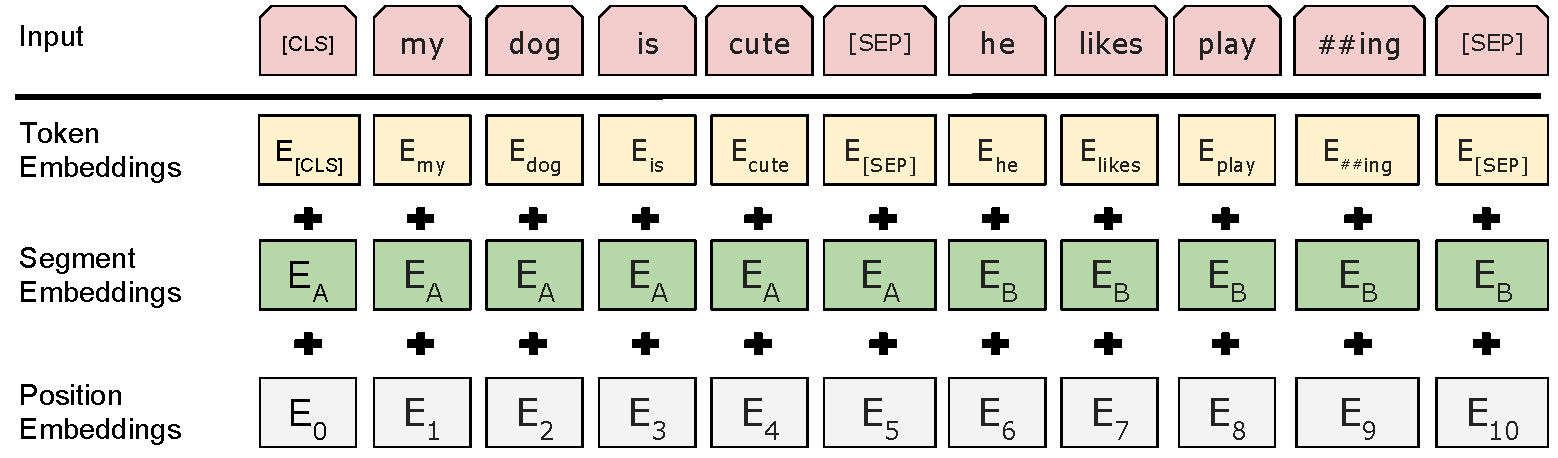
\includegraphics[width=.9\linewidth]{img/Input_Emebeddings.pdf}
\caption{\label{fig:inputemebeddings}Пример ввода текста в модель}
\end{figure}

При обучении модель выполняет на 2 задания:
\begin{enumerate}
\item Предсказание слова в предложении

Поскольку стандартные языковые модели либо смотрят текст слева направо или справа налево \ref{fig:BERT_comparisons}, как ELMo\autocite{peters_deep_2018} и GPT\autocite{radford_language_2019}, они не подходят под некоторые типы заданий. Так как BERT двунаправленный, у каждого слова можно посмотреть его контекст, что позволит предсказать замаскированное слово.

\begin{figure}[h]
\centering
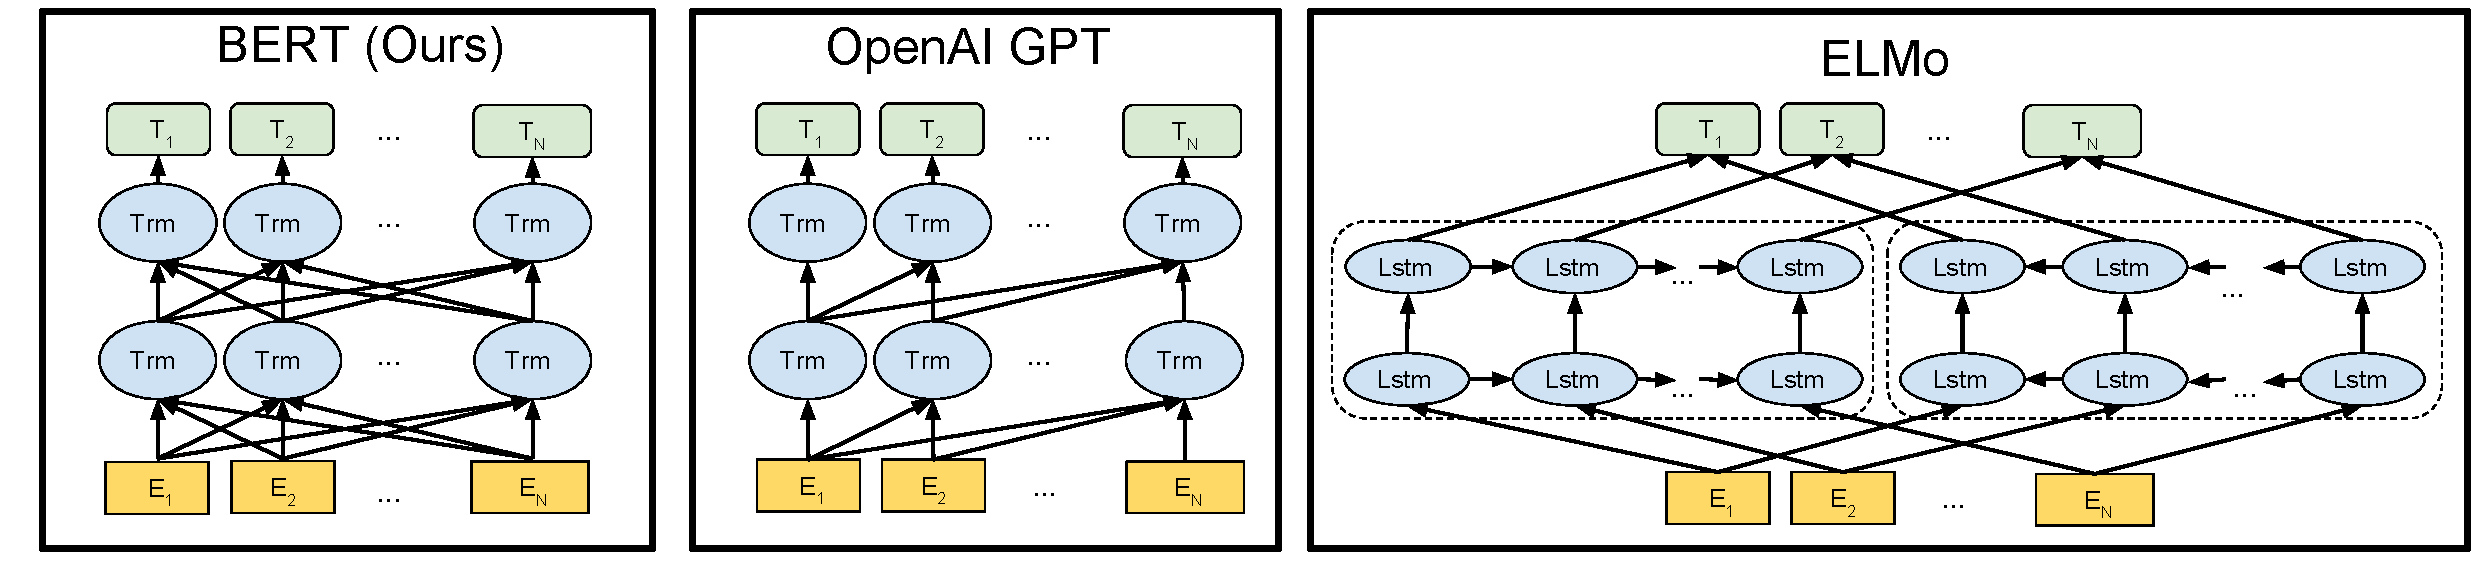
\includegraphics[width=.9\linewidth]{img/BERT_comparisons.pdf}
\caption{\label{fig:BERT_comparisons}Сравнение принципов работы BERT, ELMo, GPT}
\end{figure}

Это задание обучается следующим образом -- 15\% случайных слов заменяются в каждом предложении на специальный токен \texttt{[MASK]}, а затем предсказываются на основании контекста. Однако иногда слова заменяются не на специальны токена, в 10\% заменяются на случайный токен и еще в 10\% заменяются на случайное слово.

\item Предсказание следующего предложения

Для того чтобы обучить модель, которая понимает отношения предложений, она предсказывает, идут ли предложения друг за другом. Для этого с 50\% вероятностью выбирают предложения, которые находятся рядом и наоборот. Пример ввода пары предложений в модель \ref{fig:bert_pretrainin}.

\begin{figure}[hbp]
\centering
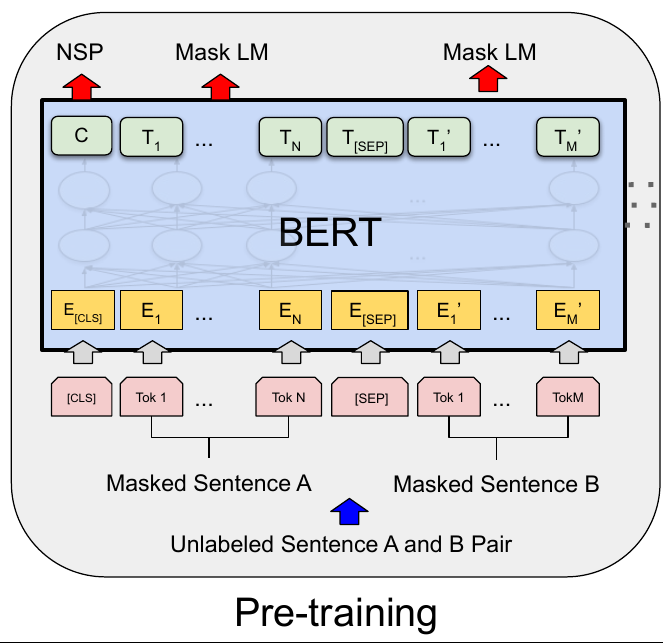
\includegraphics[width=0.6\textwidth]{img/bert_pretrainin.png}
\caption{\label{fig:bert_pretrainin}Схемам работы BERT}
\end{figure}
\end{enumerate}
\subsection{Sentence BERT}
\label{sec:org21460a1}
Sentense BERT \autocite{reimers_sentence-bert_2019} -- это модификация предобученных моделей BERT, которая использует 2 модели BERT, затем усреднят их выходы, а после с помощью функции ошибки выдаёт результат. Схема работы модели \ref{fig:sbert}.
\begin{figure}[h!]
\centering
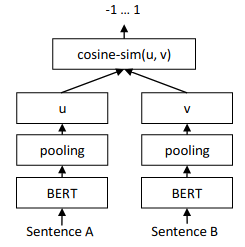
\includegraphics[width=0.6\textwidth]{img/sbert.png}
\caption{\label{fig:sbert}Схема работы SBERT}
\end{figure}
Основное преимущество данной модели над классическим BERT: эмбеддинги предложений можно сравнивать друг с другом независимо и не пересчитывать их пару каждый раз. Например, если для поиска похожих предложений из 10000 для обычного BERT потребуется 50 миллионов вычислений различных пар предложений, и это займёт 50 часов, то Sentense BERT рассчитает эмбеддинг каждого предложения отдельно, потом их сравнит. Такой способ рассчета ускоряет работу программы до 5 секунд.
\section{Анализ требований к системе}
\label{sec:org9e2a8b3}
Исходя из интервью с пользователями система должна уметь:
\begin{enumerate}
\item Показывать историю изменений индекса с возможностью фильтровать по:
\begin{enumerate}
\item годам;
\item отраслям компаний, с возможностью множественного выбора;
\item компаниям, с возможностью множественного выбора;
\item моделям, с возможностью множественного выбора;
\item источникам, с возможностью множественного выбора.
\end{enumerate}
\item Агрегировать значения индекса по годам и кварталам;
\item Анализировать тексты для построения индекса этичности;
\item Иметь возможность добавления анализа текста несколькими вариантами;
\item Сохранять тексты для последующего анализа другими методами;
\item Система должна собирать данные с сайтов banki.ru, sravni.ru и комментарии из групп {}<<вконтаке>>{};
\item На сайте должен быть график, который показывать изменение индекса этичности компаний и количества собранных отзывов по разным источникам.
\item Для расчета индекса этичности компаний на основании рецензий должна использоваться формула\ref{eq:ethics}:
\end{enumerate}

\begin{equation}
\label{eq:ethics}
\begin{aligned}
\text{Base index} &= \frac{\text{positive} - \text{negative}}{\text{positive} + \text{negative}} \\
\text{Std index} &= \sqrt{\frac{\text{positive}}{\text{negative} \cdot (\text{positive} + \text{negative})^{3}} + \frac{\text{negative}}{\text{positive} \cdot (\text{positive} + \text{negative})^{3}}} \\
\text{Index} &= ({2\cdot({\text{Base index}}-{\text{Mean index}} > 0) - 1})\cdot\\
            &{max\left(\left|{\text{Base index}}-{\text{Mean index}}\right|-{\text{Std index}}, 0\right)}
\end{aligned}
\end{equation}

\(positive\) -- количество позитивных предложений,

\(negative\) -- количество негативных предложений,

\(Mean\ index\) -- среднее значения для пар источник сбора данных и модели, которая обрабатывала предложения.

На основе описания функциональных требований была создана диаграмма вариантов использования, которая представлена на рисунке \ref{fig:usecasefull}.
\begin{figure}[h!]
\centering
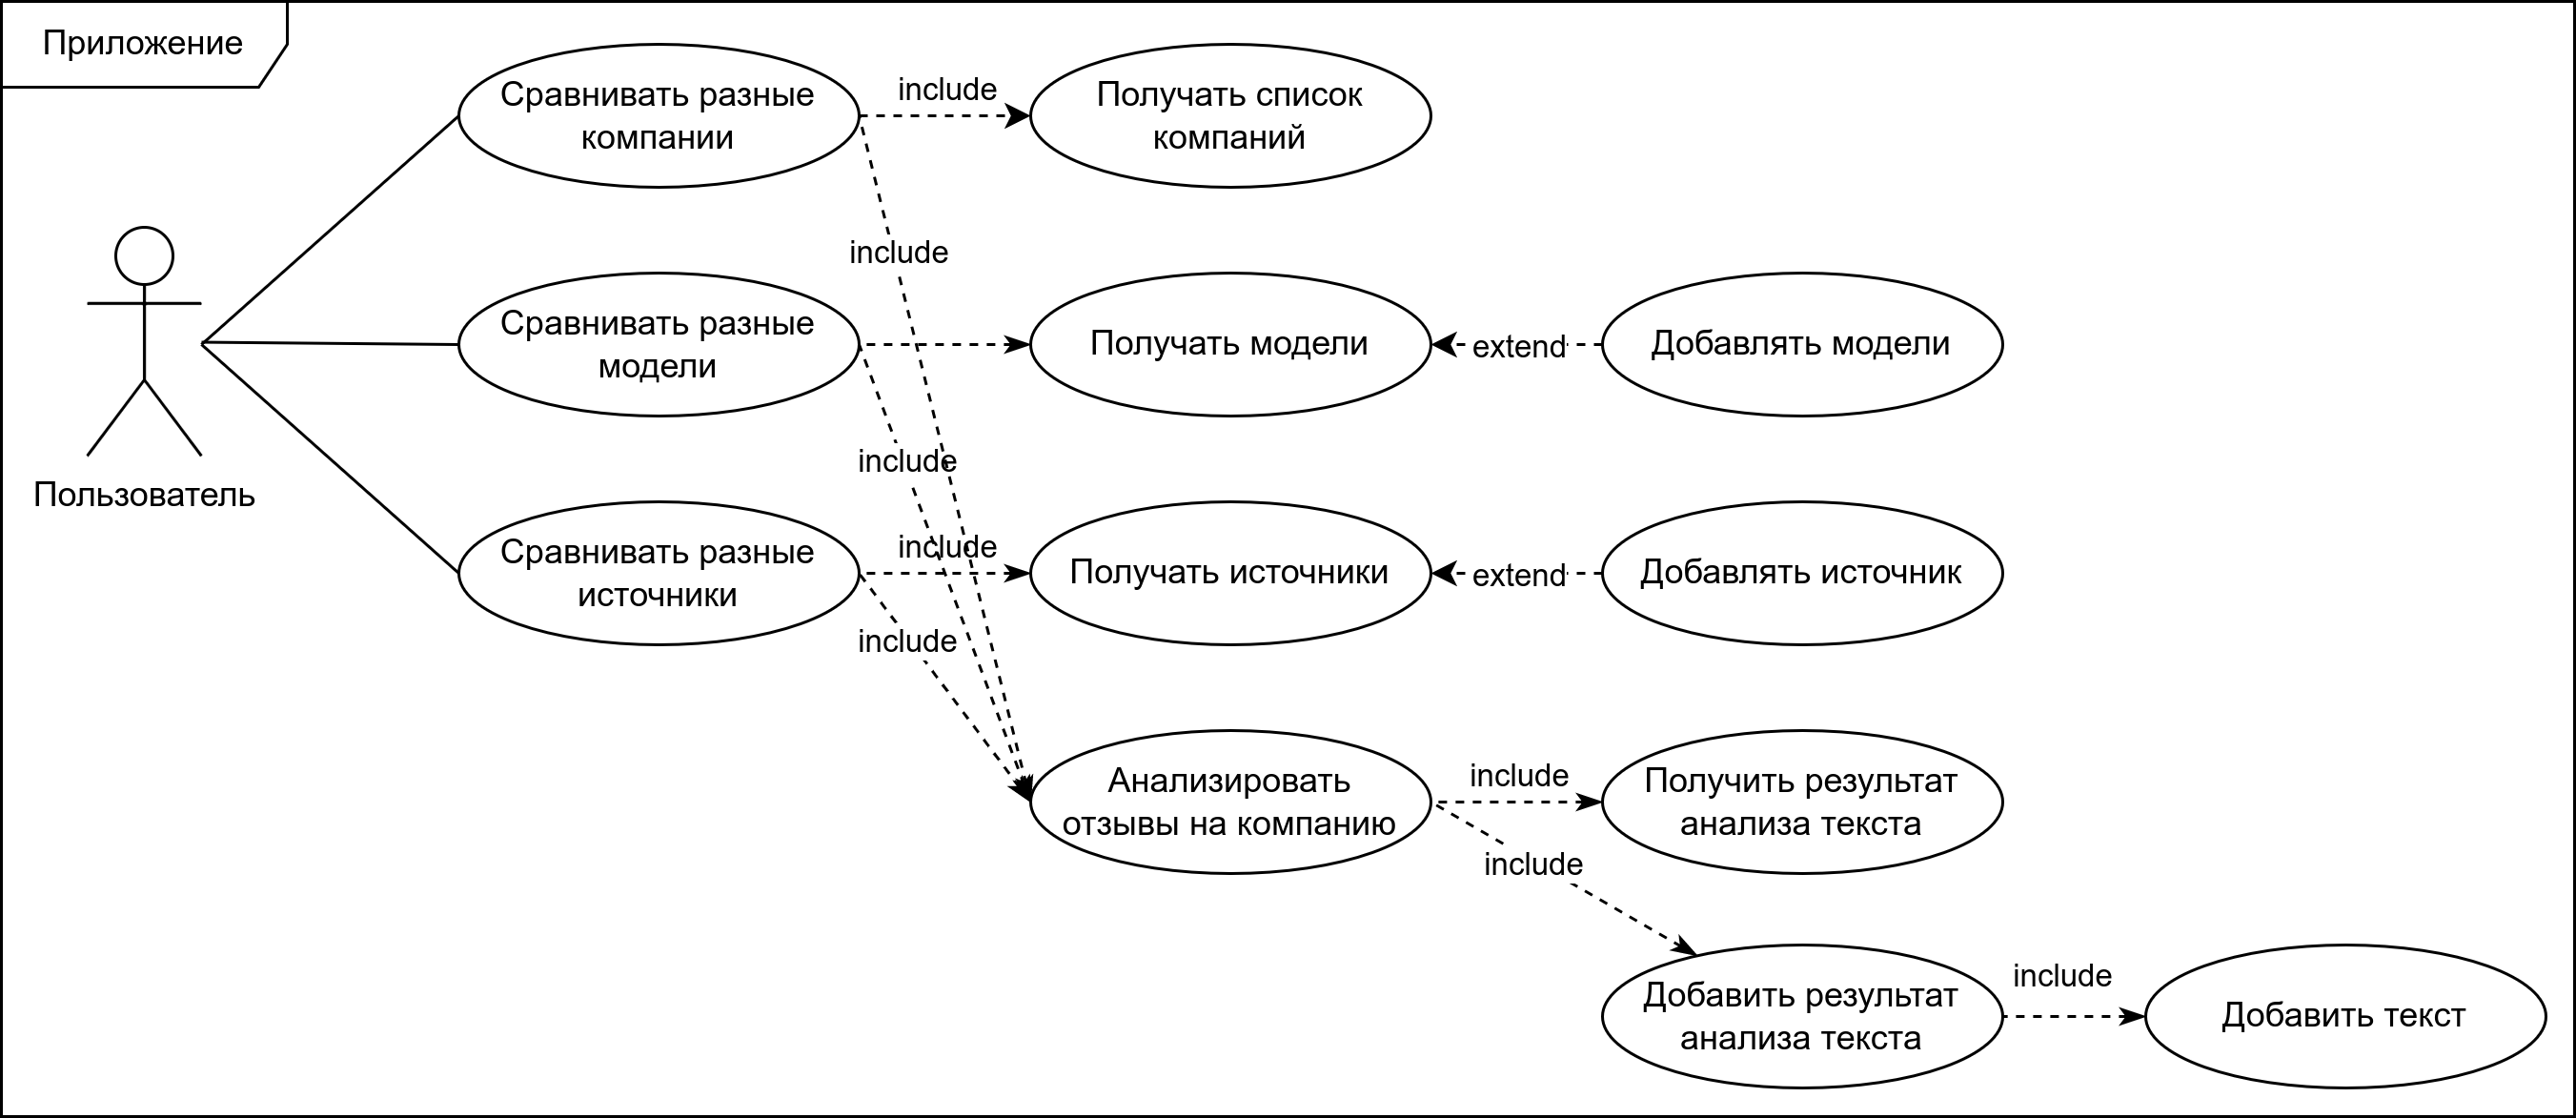
\includegraphics[width=\textwidth]{img/use-case.png}
\caption{\label{fig:usecasefull}Диаграмма вариантов использования}
\end{figure}

Также были получены нефункциональные требования:
\begin{enumerate}
\item построение графика не должно занимать больше секунды;
\item данные должны собираться автоматически;
\item данные должны обрабатываться автоматически;
\item система должны способна работать с большим объемом информации;
\item система должна быть стабильна.
\end{enumerate}
\section{Выбор технологий для разработки}
\label{sec:orgc35e1b4}
Для реализации этой системы будет использоваться язык Python. Для этого языка разработано много библиотек, которые позволят быстро реализовать нейротропные алгоритмы обработки естественного языка, в частности в этом проекте будет использоваться Pytorch\autocite{paszke_pytorch_2019} и HuggingFace\autocite{wolf_transformers_2020}, и собирать данные с сайтов. Для реализации API будет использоваться FastAPI, что позволит разрабатывать API с автоматической документацией.

Хранение данных будет использоваться объектно-реляционная система управления базами данных PostgreSQL, что позволит обрабатывать большие объемы данных. Для работы с ней будет использоваться Code first подход, с помощью Python библиотек Sqlalchemy и Alembic для изменения схемы данных (миграций).

Для клиентской части приложения будет использоваться библиотека React.
\section{Выводы главы}
\label{sec:orgd74ba0e}
По итогам анализа предметной области, можно сделать вывод о том, что определение этичности компаний является важной задачей, которую можно автоматизировать с помощью алгоритмов машинного обучения. Анализ оценок этичности компаний позволяет понять, какие факторы необходимо учитывать при разработке алгоритмов. Обзор существующих решений показал, что некоторые из них имеют свои преимущества и недостатки, и может потребоваться разработка нового средства, учитывающего особенности задачи. Анализ алгоритмов помогает выбрать наиболее подходящие алгоритмы для поиска полезной информации в текстах. Наконец, анализ требований к системе позволяет определить необходимые функциональные и нефункциональные требования, которые будут учитываться при разработке решения. В целом, эти аналитические пункты помогут определить оптимальный подход к решению задачи определения этичности компаний.
\chapter{Проектирование системы}
\label{sec:org3f1ca05}
В данной главе определена общая архитектура системы и каждого микросервиса, осуществлено проектирование баз данных, API микросервисов для модуля анализа для универсальной рекомендательной системы.
\section{Проектирование архитектуры системы}
\label{sec:org944e46d}
Система будет разделена на отдельные независимые компоненты (микросервисы), что позволит ей быть надежной, если в какой-то части системы будут сбои, то остальная часть системы продолжит работать, и масштабируемой, легко добавлять новые компоненты. Каждый микросервис системы будет представлять собой docker container, которые будут управляться с помощью docker compose. Каждый сервис будет реализовывать отдельный компонент бизнес-логики и коммуницировать с другими компонентами через HTTP API.

Было выделено 5 главных компонента бизнес логики:
\begin{enumerate}
\item Работа с базой данных -- это HTTP API, который обеспечивает возможность сохранения и получения данных из базы данных. Данный компонент принимает запросы на сохранение данных, получение информации из базы данных и возвращает результаты обработки этих запросов.
\item Сбор данных -- компонент, который отвечает за сбор информации с нескольких источников. Для этого используется несколько независимых сборщиков данных, которые работают с различными сайтами и другими источниками.
\item Обработка данных -- данный компонент содержит несколько моделей, которые используются для анализа данных. Эти модели производят различные виды анализа, от простой фильтрации и сортировки до более сложных операций анализа и прогнозирования.
\item Агрегирование данных -- этот компонент отвечает за агрегацию обработанных данных в единый индекс. Данный индекс может быть использован для удобного представления полученных результатов в виде отчетов и графиков.
\item Сайт -- этот компонент будет отображать агрегированную информацию.
\end{enumerate}

Результат архитектуры системы на рис. \ref{fig:architecture}.

\begin{figure}[h!]
\centering
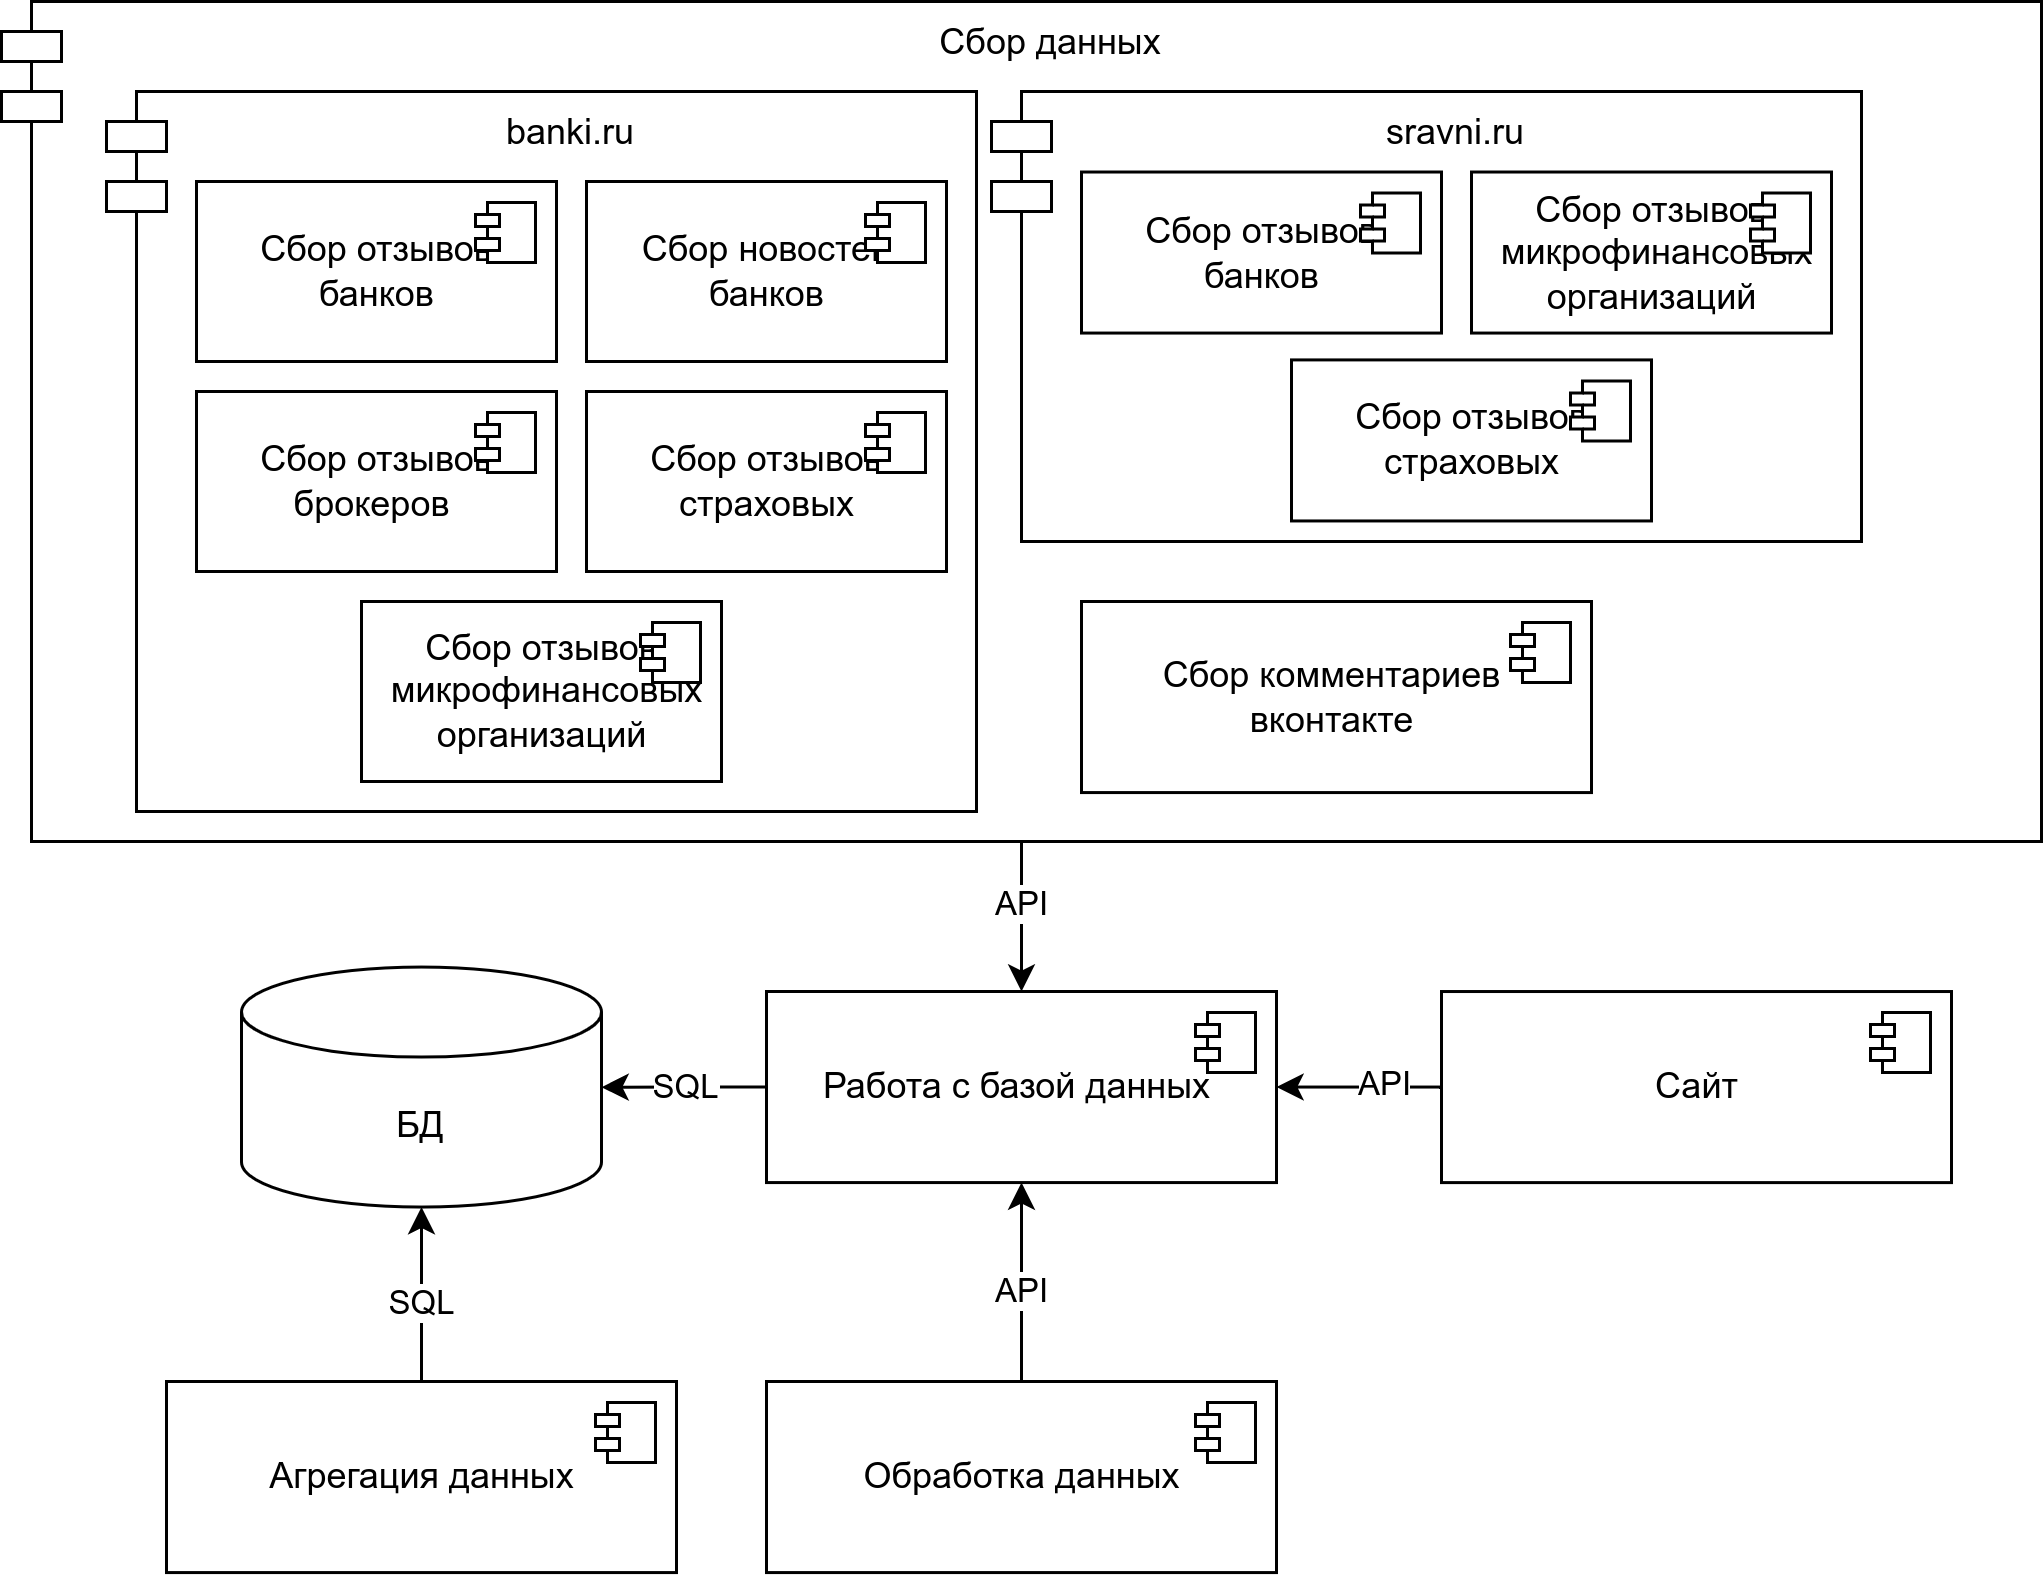
\includegraphics[width=0.8\textwidth]{img/architecture.png}
\caption{\label{fig:architecture}Диаграмма архитектуры системы}
\end{figure}

Сервис для работы с базой данных, который будет обеспечивать сохранение и получение информации из различных сервисов сбора и обработки данных, а также сайтов. Для этого будет предоставлен API, который будет использоваться для отправки и получения данных.

Сервисы сбора данных будут отправлять собранные тексты в формате JSON на сервис работы с базой данных с помощью HTTP запросов. Кроме того, информация, необходимая для сбора данных, будет храниться в базах данных соответствующих сервисов.

Сервис агрегации данных будет периодически обновлять базу данных один раз в день для обеспечения актуальности данных.

Сервис сбора данных будет включать несколько моделей машинного обучения, которые будут использоваться для анализа данных, полученных из сервиса сбора данных. После обработки данных, результаты будут отправляться обратно в сервис сбора данных.

Сайт будет получать данные из сервиса работы с базой данных.
\section{Проектирование базы данных}
\label{sec:orgebdf924}
\subsection{Проектирование основной базы данных}
\label{sec:org617ebb8}
На основании требований была разработана следующая схема базы данных:

Таблица сфер компаний, чтобы можно было фильтровать различные сферы компаний и смотреть как меняется этичность сферы в целом.

\begin{center}
\begin{longtblr}[caption={Таблица сфера компании\label{tbl:company_type} }]{colspec={|X[2,l]|X[1,l]|X[3,l]|},rowhead = 1,hlines}
\textbf{Название} & \textbf{Тип} & \textbf{Описание}\\[0pt]
Идентификатор & Целое & Уникальный идентификатор\\[0pt]
Сфера компании & Строка & \\[0pt]
\end{longtblr}
\end{center}

\begin{center}
\begin{longtblr}[caption={Таблица компании\label{tbl:companies}}]{colspec={|X[l]|X[l]|X[l]|},rowhead = 1,hlines}
\textbf{Название} & \textbf{Тип} & \textbf{Описание}\\[0pt]
Идентификатор & Целое & Уникальный идентификатор\\[0pt]
Название компании & Строка & \\[0pt]
Описание компании & Строка & Дополнительное поле для сохранения вспомогательной информации о компании\\[0pt]
Лицензия компании & Строка & По лицензии компаний может будет сопоставлять компании на разных сайтах\\[0pt]
Код сферы компании & Целое & Внешний ключ из таблицы Сфера компании\\[0pt]
\end{longtblr}
\end{center}

\begin{center}
\begin{longtblr}[caption={Таблица тип источников\label{tbl:source_type}}]{colspec={|X[l]|X[l]|X[l]|},rowhead = 1,hlines}
\textbf{Название} & \textbf{Тип} & \textbf{Описание}\\[0pt]
Идентификатор & Целое & Уникальный идентификатор\\[0pt]
Название типа источника & Строка & \\[0pt]
\end{longtblr}
\end{center}

\begin{center}
\begin{longtblr}[caption={Таблица источники\label{tbl:sources} }]{colspec={|X[l]|X[l]|X[l]|},rowhead = 1,hlines}
\textbf{Название} & \textbf{Тип} & \textbf{Описание}\\[0pt]
Идентификатор & Целое & Уникальный идентификатор\\[0pt]
Сайт & Строка & Сайт источника\\[0pt]
Код типа источника & Целое & Внешний ключ из таблицы тип источника\\[0pt]
Состояние сборщика данных & JSON & Данные о текущем состояние сборщика данных, если возникнет сбой\\[0pt]
Дата последнего сбора & DateTime & Точка когда сбор данных закончился, для дальнейшего сбора данных\\[0pt]
\end{longtblr}
\end{center}

\begin{center}
\begin{longtblr}[caption={Таблица тип модели\label{tbl:model_type}}]{colspec={|X[l]|X[l]|X[l]|},rowhead = 1,hlines}
\textbf{Название} & \textbf{Тип} & \textbf{Описание}\\[0pt]
Идентификатор & Целое & Уникальный идентификатор\\[0pt]
Название модели & Строка & \\[0pt]
\end{longtblr}
\end{center}

\begin{center}
\begin{longtblr}[caption={Таблица модели\label{tbl:model}}]{colspec={|X[l]|X[l]|X[l]|},rowhead = 1,hlines}
\textbf{Название} & \textbf{Тип} & \textbf{Описание}\\[0pt]
Идентификатор & Целое & Уникальный идентификатор\\[0pt]
Название модели & Строка & \\[0pt]
Код типа модели & Целое & Внешний ключ на таблицу тип модели\\[0pt]
\end{longtblr}
\end{center}

\begin{center}
\begin{longtblr}[caption={Таблицы текст\label{tbl:text}}]{colspec={|X[l]|X[l]|X[l]|},rowhead = 1,hlines}
\textbf{Название} & \textbf{Тип} & \textbf{Описание}\\[0pt]
Идентификатор & Целое & Уникальный идентификатор\\[0pt]
Ссылка & Строка & Ссылка на текст\\[0pt]
Код источника & Целое & Внешний ключ из таблицы источники\\[0pt]
Дата текста & DateTime & Время публикации текста\\[0pt]
Заголовок & Строка & Заголовок текста\\[0pt]
Код компании & Целое & Внешний ключ на компанию\\[0pt]
Количество комментариев & Целое & \\[0pt]
\end{longtblr}
\end{center}

Так как Bert на вход принимает отдельные предложения, было решено сделать для них отдельную таблицу.

\begin{center}
\begin{longtblr}[caption={Таблица предложений\label{tbl:sentence}}]{colspec={|X[l]|X[l]|X[l]|},rowhead = 1,hlines}
\textbf{Название} & \textbf{Тип} & \textbf{Описание}\\[0pt]
Идентификатор & Целое & Уникальный идентификатор\\[0pt]
Код текста & Целое & Внешний ключ из таблицы тексты\\[0pt]
Предложение & Строка & \\[0pt]
Номер предложения & Целое & Порядковый номер предложения в тексте\\[0pt]
\end{longtblr}
\end{center}

\begin{center}
\begin{longtblr}[caption={Таблица результатов анализа текстов\label{tbl:text_result}}]{colspec={|X[l]|X[l]|X[l]|},rowhead = 1,hlines}
\textbf{Название} & \textbf{Тип} & \textbf{Назначение}\\[0pt]
Идентификатор & Целое & Уникальный идентификатор\\[0pt]
Код предложения & Целое & Внешний ключ из таблицы предложения\\[0pt]
Код модели & Целое & Внешний ключ из таблицы модели\\[0pt]
Результат & Вещественный массив & Результат работы модели\\[0pt]
Обработано & Логическое & Показатель, обработано ли предложение или нет\\[0pt]
\end{longtblr}
\end{center}

Диаграмма полученной схемы базы данных рис. \ref{fig:database}.
\subsection{Проектирование базы данных для агрегации}
\label{sec:org5a99538}
При сборе функциональных требований было выявлено, что надо быстро показывать количество собранных отзывов и индекс компаний.

Обработанные данные из таблицы\textasciitilde{}\ref{tbl:text_result} агрегируются для каждого квартала и для расчета индекса по формуле \ref{eq:ethics} будут добавлены дополнительные колонки.
\begin{center}
\begin{longtblr}[caption={Таблица для расчета и показа индекса\label{tbl:index_calc}}]{colspec={|X[2,l]|X[1,l]|X[3,l]|},rowhead = 1,hlines}
\textbf{Название} & \textbf{Тип} & \textbf{Описание}\\[0pt]
Идентификатор & Целое & Уникальный идентификатор\\[0pt]
Год & Целое & Год за который был агрегирован индекс\\[0pt]
Квартал & Целое & Квартал за который был агрегирован индекс\\[0pt]
Название модели & Строка & \\[0pt]
Сайт источника & Строка & \\[0pt]
Тип источника & Строка & \\[0pt]
Название банка & Строка & \\[0pt]
Код банка & Целое & Для запросов через API\\[0pt]
Нейтральный & Целое & Количество нейтральных предложений за период\\[0pt]
Позитивный & Целое & Количество позитивных предложений за период\\[0pt]
Негативный & Целое & Количество негативных предложений за период\\[0pt]
Базовый индекс & Вещественное & Индекс для расчета итогового индекса\\[0pt]
Средний индекс & Вещественное & Индекс для расчета итогового индекса\\[0pt]
Std индекс & Вещественное & Индекс для расчета итогового индекса\\[0pt]
Индекс & Вещественное & Рассчитанный индекс\\[0pt]
\end{longtblr}
\end{center}

Собранные отзывы из таблицы\textasciitilde{}\ref{tbl:text} агрегируются для каждого месяца и будет собираться количество собранных отзывов за месяц.
\begin{center}
\begin{longtblr}[caption={Таблица для расчета и показа индекса\label{tbl:index_calc}}]{colspec={|X[2,l]|X[1,l]|X[3,l]|},rowhead = 1,hlines}
\textbf{Название} & \textbf{Тип} & \textbf{Описание}\\[0pt]
Идентификатор & Целое & Уникальный идентификатор\\[0pt]
Дата & DateTime & \\[0pt]
Квартал & Целое & Квартал за который был агрегирован индекс\\[0pt]
Тип источника & Строка & \\[0pt]
Сайт & Строка & \\[0pt]
Количество отзывов & Целое & \\[0pt]
\end{longtblr}
\end{center}

Диаграмма полученной схемы базы данных рис. \ref{fig:database_views}.
\section{Проектирование серверной части}
\label{sec:org7c49d66}
\subsection{Модуль сбора данных}
\label{sec:org3317dcc}
\subsection{Модуль обработки данных}
\label{sec:orgfcbfc24}
\subsection{Модуль агрегации данных}
\label{sec:orga41e96c}
\section{Проектирование сборщиков данных}
\label{sec:org399978e}
\subsection{Проектирование сбора данных с banki.ru}
\label{sec:org3043f9a}
\begin{center}
\begin{longtblr}[caption={Таблица для сайта banki.ru\label{tbl:banki_ru}}]{colspec={|X[2,l]|X[1,l]|X[3,l]|},rowhead = 1,hlines}
\textbf{Название} & \textbf{Тип} & \textbf{Описание}\\[0pt]
Идентификатор & Целое & Уникальный идентификатор\\[0pt]
Идентификатор банка & Целое & Идентификатор банка в основной базе данных\\[0pt]
Имя банка & Строка & \\[0pt]
Код банка & Строка & Код банка для запросов по API\\[0pt]
\end{longtblr}
\end{center}

Диаграмма полученной схемы базы данных рис. \ref{fig:database_banki_ru}.
\subsection{Проектирование сбора данных с sravni.ru}
\label{sec:orgc55f297}
\begin{center}
\begin{longtblr}[caption={Таблица для сайта sravni.ru\label{tbl:sravni_ru}}]{colspec={|X[2,l]|X[1,l]|X[3,l]|},rowhead = 1,hlines}
\textbf{Название} & \textbf{Тип} & \textbf{Описание}\\[0pt]
Идентификатор & Целое & Уникальный идентификатор\\[0pt]
Идентификатор банка & Целое & Идентификатор банка в основной базе данных\\[0pt]
Код банка в sravni.ru & Целое & \\[0pt]
Старый код банка в sravni.ru & Целое & \\[0pt]
Псевдоним компании & Строка & \\[0pt]
Название банка & Строка & \\[0pt]
\end{longtblr}
\end{center}
Диаграмма полученной схемы базы данных рис. \ref{fig:database_sravni_ru}
\subsection{Проектирование сбора данных с vk.com}
\label{sec:org3d8734e}
\begin{center}
\begin{longtblr}[caption={Таблица для сайта vk.com\label{tbl:vk_com}}]{colspec={|X[2,l]|X[1,l]|X[3,l]|},rowhead = 1,hlines}
\textbf{Название} & \textbf{Тип} & \textbf{Описание}\\[0pt]
Идентификатор & Целое & Уникальный идентификатор\\[0pt]
Идентификатор на vk.com & Строка & \\[0pt]
Имя компании & Строка & \\[0pt]
Домен компании на vk.com & Строка & \\[0pt]
\end{longtblr}
\end{center}

Диаграмма полученной схемы базы данных рис. \ref{fig:database_vk_com}.
\section{Проектирование клиентской части}
\label{sec:org728cc1c}
\chapter{Реализация системы}
\label{sec:org2ea75e9}
\section{Реализация серверной части}
\label{sec:orge5c23ba}
\subsection{Реализация API}
\label{sec:org22e2e62}
\subsection{Реализация парсера banki.ru}
\label{sec:org4ff0bee}
\subsection{Реализация парсера sravni.ru}
\label{sec:orgfc3402f}
\subsection{Реализация модуля обработки текста}
\label{sec:org3939f08}
\subsection{Дообучение модели}
\label{sec:orgfcc7cfb}
\section{Реализация клиентской части}
\label{sec:orgbe27703}
\chapter{Тестирование системы}
\label{sec:orgcb84672}
\chapter*{Заключение}
\label{sec:orgd9a6494}
\putbibliography
\appendix
% https://www.swrit.ru/doc/gost34/34.602-2020.pdf
% Сделано по гост 34.602-2020
{ % чтобы в главном тексте не сбрасывались заголовки
%%%%%%%%%%%%%%%%%%%%% переопределение секций чтобы было 1.1. вместо А.1.1.
\renewcommand*{\thesection}{\arabic{section}}
\titleformat{\section}{\large\bfseries}{\thesection.}{4pt}{}

\renewcommand*{\thesubsection}{\arabic{section}.\arabic{subsection}}
\titleformat{\subsection}{\large\bfseries}{\thesubsection.}{4pt}{}

\renewcommand*{\thesubsubsection}{\arabic{section}.\arabic{subsection}.\arabic{subsubsection}}
\titleformat{\subsubsection}{\normalsize\bfseries}{\thesubsubsection.}{4pt}{}
\setcounter{secnumdepth}{4}

%%%%%%%%%%%%%%%%%%%%%%%%%% 5
{ % для титульного листа
  \chapter*{ПРИЛОЖЕНИЕ А Техническое задание на разрабатываемую систему}\label{tz_chap}

\stepcounter{chapter}
\thispagestyle{empty}
\centering

\begin{flushright}
  \MakeUppercase{Утверждено}

  A.B.00001-01 ТЗ 01
\end{flushright}

\vfill

\textbf{\MakeUppercase{Система для автоматического сбора, анализа и визуализации информации по этичности компаний}}

\textbf{Техническое задание}

\textbf{\textit{Лист утверждения}}

\vbox{
  \parbox{6cm}{
    \begin{sideways}
      \setlength\arrayrulewidth{2pt}
      \begin{tabular}{|c|c|c|c|c|}
        \hline
        Инв. № подл. & Подпись и дата & Взам. инв. № & Инв. № дубл. & Подпись и дата \\
        \hline
                     &&&&\\
        \hline
      \end{tabular}
    \end{sideways}
  }
  \hfill
  \parbox{9.4cm}{
    \begin{flushright}
      \begin{minipage}[t]{0.4\textwidth}
        Руководитель разработки

        \vspace{3mm}
        \makebox[6cm][r]{\hrulefill~Бузмаков~А.В.}
        \makebox[6cm][r]{<<\rule{7mm}{0.4pt}>>\hrulefill~\the\year}
      \end{minipage}
    \end{flushright}
    \vspace{10mm}
    \begin{flushright}
      \begin{minipage}[t]{0.4\textwidth}
        Исполнитель

        \vspace{3mm}
        \makebox[6cm][r]{\hrulefill~Соломатин~Р.И.}
        \makebox[6cm][r]{<<\rule{7mm}{0.4pt}>>\hrulefill~\the\year}
      \end{minipage}
    \end{flushright}
  }
}
\newpage
}
\section{Общие сведения}
Наименование программы – <<Система для автоматического сбора, анализа и визуализации информации по этичности компаний>> (далее – <<Система>>). Основная функция системы - сбор и анализ данных из различных источников, включая новостные сайты, социальные сети, отзывы о компаниях и другие открытые источники данных. Система использует алгоритмы машинного обучения и обработки естественного языка для автоматической обработки данных и определения этичности компаний.

Система также предоставляет визуализацию данных в виде графиков и диаграмм, позволяя пользователям легко понять и сравнивать данные по разным компаниям. Кроме того, система может предоставлять аналитические отчеты и рекомендации по улучшению этичности компаний на основе собранных данных.

Система разрабатывается в рамках выполнения выпускной квалификационной работы. Основанием для разработки являются:
\begin{itemize}
  \item Положение о курсовой и выпускной квалификационной работе студентов, обучающихся по программам бакалавриата, специалитета и магистратуры в Национальном исследовательском университете <<Высшая школа экономики>>, утвержденным ученым советом НИУ ВШЭ (протокол от 28.11.2014 № 08), с изменениями от 29.03.2016;
  \item Правила подготовки выпускной квалификационной работы студентов основной образовательной программы бакалавриата <<Программная инженерия>> по направлению подготовки 09.03.04. Программная инженерия, утвержденные протоколом ученого совета НИУ ВШЭ – Пермь от 19.11.2020 № 8.2.1.7-10/10.
\end{itemize}

\section{Цели и назначение создания автоматизированной системы}

\subsection{Цели создания АС}
Целью создания системы является получение инструмента который позволит анализировать компании на основании их этичности, соответствующего следующим требованиям:
\begin{itemize}
  \item Показывать историю изменений индекса с возможностью фильтровать по
        \begin{itemize}
          \item годам;
          \item отраслям компаний, с возможностью множественного выбора;
          \item компаниям, с возможностью множественного выбора;
          \item моделям, с возможностью множественного выбора;
          \item источникам, с возможностью множественного выбора.
        \end{itemize}
  \item Агрегировать значения индекса по годам и кварталам;
  \item Анализировать тексты для построения индекса этичности;
  \item Иметь возможность добавления анализа текста несколькими вариантами;
  \item Сохранять тексты для последующего анализа другими методами;
  \item Система должна собирать данные с сайтов banki.ru, sravni.ru и комментарии из групп {}<<вконтаке>>{};
  \item На сайте должен быть график, который показывать изменение индекса этичности компаний и количества собранных отзывов по разным источникам.
  \item Для расчета индекса этичности компаний на основании рецензий должна использоваться формула\ref{eq:ethics_tz}:
        \begin{equation}
          \label{eq:ethics_tz}
          \begin{aligned}
            \text{Base index} &= \frac{\text{positive} - \text{negative}}{\text{positive} + \text{negative}} \\
            \text{Std index} &= \sqrt{\frac{\text{positive}}{\text{negative} \cdot (\text{positive} + \text{negative})^{3}} + \frac{\text{negative}}{\text{positive} \cdot (\text{positive} + \text{negative})^{3}}} \\
            \text{Index} &= ({2\cdot({\text{Base index}}-{\text{Mean index}} > 0) - 1})\cdot\\
                              &{max\left(\left|{\text{Base index}}-{\text{Mean index}}\right|-{\text{Std index}}, 0\right)}
          \end{aligned}
        \end{equation}

        \(positive\) -- количество позитивных предложений,

        \(negative\) -- количество негативных предложений,

        \(Mean\ index\) -- среднее значения для пар источник сбора данных и модели, которая обрабатывала предложения.
\end{itemize}


\subsection{Назначение АС}
Система предназначена для собора и анализа отзывы потребителей с различных веб-сайтов, с помощью алгоритмов обработки естественного языка.
\section{Характеристика объекта автоматизации}
Система автоматизирует процесс анализа этичности компаний.
\section{Требования к автоматизированной системе}
Требования к АС:
\begin{enumerate}
  \item построение графика не должно занимать больше секунды;
  \item данные должны собираться автоматически;
  \item данные должны обрабатываться автоматически;
  \item система должны способна работать с большим объемом информации;
  \item система должна быть стабильна.
\end{enumerate}
\subsection{Требования к структуре АС в целом}
Должно быть несколько модулей, которые общаются между собой с помощью HTTP API:
\begin{itemize}
  \item сборщики данных;
  \item взаимодействие с базой данных(API);
  \item сайт;
  \item модели для обработки данных.
\end{itemize}
Все подсистемы должны быть в Docker контейнерах.
\subsection{Требования к функциям (задачам), выполняемым АС}
\subsubsection{Требования к API}
Система взаимодействия с базой данных должна выполнять функции:
\begin{itemize}
  \item хранить информацию о компаниях;
  \item модель должна отдавать информацию о компаниях из разных сфер;
  \item хранить информацию о разных источниках;
  \item добавлять различные источники;
  \item получать отзывы и разбивать их на предложения;
  \item иметь возможность отдавать необработанные предложения в зависимости от модели;
  \item сохранять информацию о моделях;
  \item сохранять результат обработки предложений;
  \item агрегировать результат обработки моделей для каждого квартала;
  \item хранить информацию о состоянии сборщиков данных, если у них возникнут проблемы;
  \item отдавать информацию об индексе менее, чем за минуту;
  \item рассчитывать индекс на основе полученных результатов обработки предложений.
\end{itemize}
\subsubsection{Требования к сборщикам данных}
Сборщики данных должны выполнять функции:
\begin{itemize}
  \item собирать отзывы пользователей ежедневно;
  \item собранные отзывы отправлять на API.
\end{itemize}
\subsubsection{Требования к моделям}
Модели должны выполнять функции:
\begin{itemize}
  \item обрабатывать отзывы пользователей ежедневно;
  \item обработанные отзывы отправлять на API.
\end{itemize}
\subsection{Требования к видам обеспечения АС}
\subsubsection{Требования к лингвистическому обеспечению}
Система должна соответствовать следующим требованиям:
\begin{itemize}
  \item Программный код должен быть реализован на языке Python;
  \item Документация к программе должна быть на русском языке. Других языков не планируется.
\end{itemize}
\subsubsection{Требования к программного обеспечению}
Система должна использовать:
\begin{itemize}
  \item Для разработки API следует использовать библиотеку FastAPI;
  \item Для взаимодействия с базой данных должна использоваться библиотека SQLAlchemy, а для миграций Alembic;
  \item Сборщики данных должны собирать информацию с помощью библиотеки запросов
        requests и для работы с HTML Beautiful Soup;
  \item Для нейросетевых моделей должен использоваться Pytorch;
  \item Для клиентской части будет использоваться библиотека React.
\end{itemize}
\subsubsection{Требования к техническому обеспечению}
Для работы приложения необходим сервер, который обладает следующими параметрами:
\begin{itemize}
  \item Процессор с тактовой частотой не ниже 3 ГГц и 8 ядрами;
  \item Операционная система Ubuntu 22.04 и выше;
  \item Docker 20.10.23 и выше.
  \item Графическая карта NVIDIA GTX 3080;
  \item Оперативная память не менее 16 Гб;
  \item Доступное место на жестком диске не менее 100 Гб;
\end{itemize}
\subsubsection{Требования к информационному обеспечению}
Система должна соответствовать следующим требованиям:
\begin{itemize}
  \item Система должна использовать PostgreSQL;
  \item Сервисы между собой должны взаимодействовать при помощи HTTP;
  \item Для базы данных должен всегда быть резервная копия данных.
\end{itemize}

\subsection{Общие технические требования к АС}
\subsubsection{Требования к численности и квалификации персонала}
Для разработки системы требуется программист со средней квалификацией. Для
работы с конечной системой (сайтом), не требуется высокой квалификации, поэтому
пользователь с ней справится пользователь, который пользуется сайтами.
\subsubsection{Требования к надежности}
Надежность системы зависит от надежности функционирования сервера. Устойчивое
функционирование программы будет обеспечено с помощью:
\begin{itemize}
  \item Бесперебойное питание сервера;
  \item Использованием лицензионного программного обеспечения, необходимого для
        запуска приложения, включая лицензионную операционную систему;
  \item Регулярным выполнением рекомендаций Министерства труда и социального развития РФ, изложенных в Постановлении от 23 июля 1998 г. <<Об утверждении межотраслевых типовых норм времени на работы по сервисному обслуживанию ПЭВМ и оргтехники и сопровождению программных средств>>;
  \item Регулярным выполнением требований ГОСТ 51188-98 <<Защита информации. Испытания программных средств на наличие компьютерных вирусов>>;
\end{itemize}
Время восстановление системы будет до 10 минут с момента сбоя.
\subsubsection{Требования по сохранности информации при авариях}
Отказы как самой системы, так и ее отдельных функций, могут привести к
аварийному завершению работы программы, однако при перезапуске программы ее
функциональность не должна пострадать. При таких сбоях программы база данных не
должна пострадать. Дополнительно все данные будут резервно копироваться на дополнительную базу данных.
\section{Состав и содержание работ по созданию автоматизированной системы}
\begin{longtblr}
  [caption={Этапы реализации, контрольные точки проекта},]
  {
    colspec = {|X|X|X|},
    rowhead = 1,
    hlines,
  }
  % BEGIN RECEIVE ORGTBL stages
\textbf{Основной этап} & Подэтап & \textbf{Крайний срок}\\[0pt]
Анализ & Литературный обзор & 26.12.2022\\[0pt]
Анализ & Сравнительный анализ существующих решений & 08.01.2023\\[0pt]
Анализ & Анализ сценариев использования & 14.01.2023\\[0pt]
Анализ & Написание тех задания & 21.01.2023\\[0pt]
Проектирование & Проектирование архитектуры приложения & 14.02.2023\\[0pt]
Проектирование & Проектирование базы данных & 20.03.2023\\[0pt]
Проектирование & Проектирование графического интерфейса & 20.03.2023\\[0pt]
Проектирование & Проектирование алгоритмов машинного обучения & 20.03.2023\\[0pt]
Разработка & Разработка алгоритмов для анализа текста & 01.05.2023\\[0pt]
Разработка & Реализация серверной части & 01.05.2023\\[0pt]
Разработка & Реализация клиентской части & 01.05.2023\\[0pt]
Тестирование & Подготовка тестовых сценариев & 15.05.2023\\[0pt]
Тестирование & Функциональное тестирование & 15.05.2023\\[0pt]
Тестирование & Системное тестирование & 15.05.2023\\[0pt]
Завершение & Сдача проекта & 22.05.2023\\[0pt]
% END RECEIVE ORGTBL stages
\end{longtblr}
\begin{comment}
  #+ORGTBL: SEND stages orgtbl-to-latex
  | *Основной этап* | Подэтап                                      | *Крайний срок* |
  | Анализ          | Литературный обзор                           |     26.12.2022 |
  | Анализ          | Сравнительный анализ существующих решений    |     08.01.2023 |
  | Анализ          | Анализ сценариев использования               |     14.01.2023 |
  | Анализ          | Написание тех задания                        |     21.01.2023 |
  | Проектирование  | Проектирование архитектуры приложения        |     14.02.2023 |
  | Проектирование  | Проектирование базы данных                   |     20.03.2023 |
  | Проектирование  | Проектирование графического интерфейса       |     20.03.2023 |
  | Проектирование  | Проектирование алгоритмов машинного обучения |     20.03.2023 |
  | Разработка      | Разработка алгоритмов для анализа текста     |     01.05.2023 |
  | Разработка      | Реализация серверной части                   |     01.05.2023 |
  | Разработка      | Реализация клиентской части                  |     01.05.2023 |
  | Тестирование    | Подготовка тестовых сценариев                |     15.05.2023 |
  | Тестирование    | Функциональное тестирование                  |     15.05.2023 |
  | Тестирование    | Системное тестирование                       |     15.05.2023 |
  | Завершение      | Сдача проекта                                |     22.05.2023 |
\end{comment}

\section{Порядок разработки автоматизированной системы}
В разделе «Порядок разработки автоматизированной системы» приводят следующее:
\begin{itemize}
  \item порядок организации разработки АС;
  \item перечень документов и исходных данных для разработки АС;
  \item перечень документов, предъявляемых по окончании соответствующих этапов работ;
  \item порядок проведения экспертизы технической документации;
  \item перечень макетов (при необходимости), порядок их разработки, изготовления, испытаний, необходимость разработки на них документации, программы и методик испытаний;
  \item порядок разработки, согласования и утверждения плана совместных работ по разработке АС;
  \item порядок разработки, согласования и утверждения программы работ по стандартизации;
  \item требования к гарантийным обязательствам разработчика;
  \item порядок проведения технико-экономической оценки разработки АС;
  \item порядок разработки, согласования и утверждения программы метрологического обеспечения, программы обеспечения надежности, программы эргономического обеспечения.
\end{itemize}

\section{Порядок контроля и приемки автоматизированной системы}
Осуществление приемо-сдаточных испытаний для всей системы осуществляется на основе Программы и методики испытаний и включает:
\begin{itemize}
    \item Функциональное тестирование;
    \item Тестирование удобства эксплуатации;
    \item Оценка сгенерированных уровней.
\end{itemize}

\section{Требования к составу и содержанию работ по подготовке объекта автоматизации к вводу автоматизированной системы в действие}
\begin{longtblr}[caption={Требования к программной документации}]{colspec = {|X|X|},rowhead = 1,hlines,}
    \textbf{Название документа }          & \textbf{Краткое содержание} \\
    Текст программы \par(ГОСТ 19.401–78)  & Программный код всех модулей программы с необходимыми комментариями. \\
    Программа и методика испытаний \par(ГОСТ 19.301–79) & Требования, подлежащие проверке при испытании программы, а также порядок и методы их контроля. \\
    Техническое задание \par(34.602-2020) & Назначение и область применения программы, технические, технико-экономические и специальные требования, предъявляемые к программе, необходимые стадии и сроки разработки, виды испытаний. \\
\end{longtblr}
}

\chapter{Схема базы данных}
\label{sec:org76a6214}
\begin{figure}[h!]
\centering
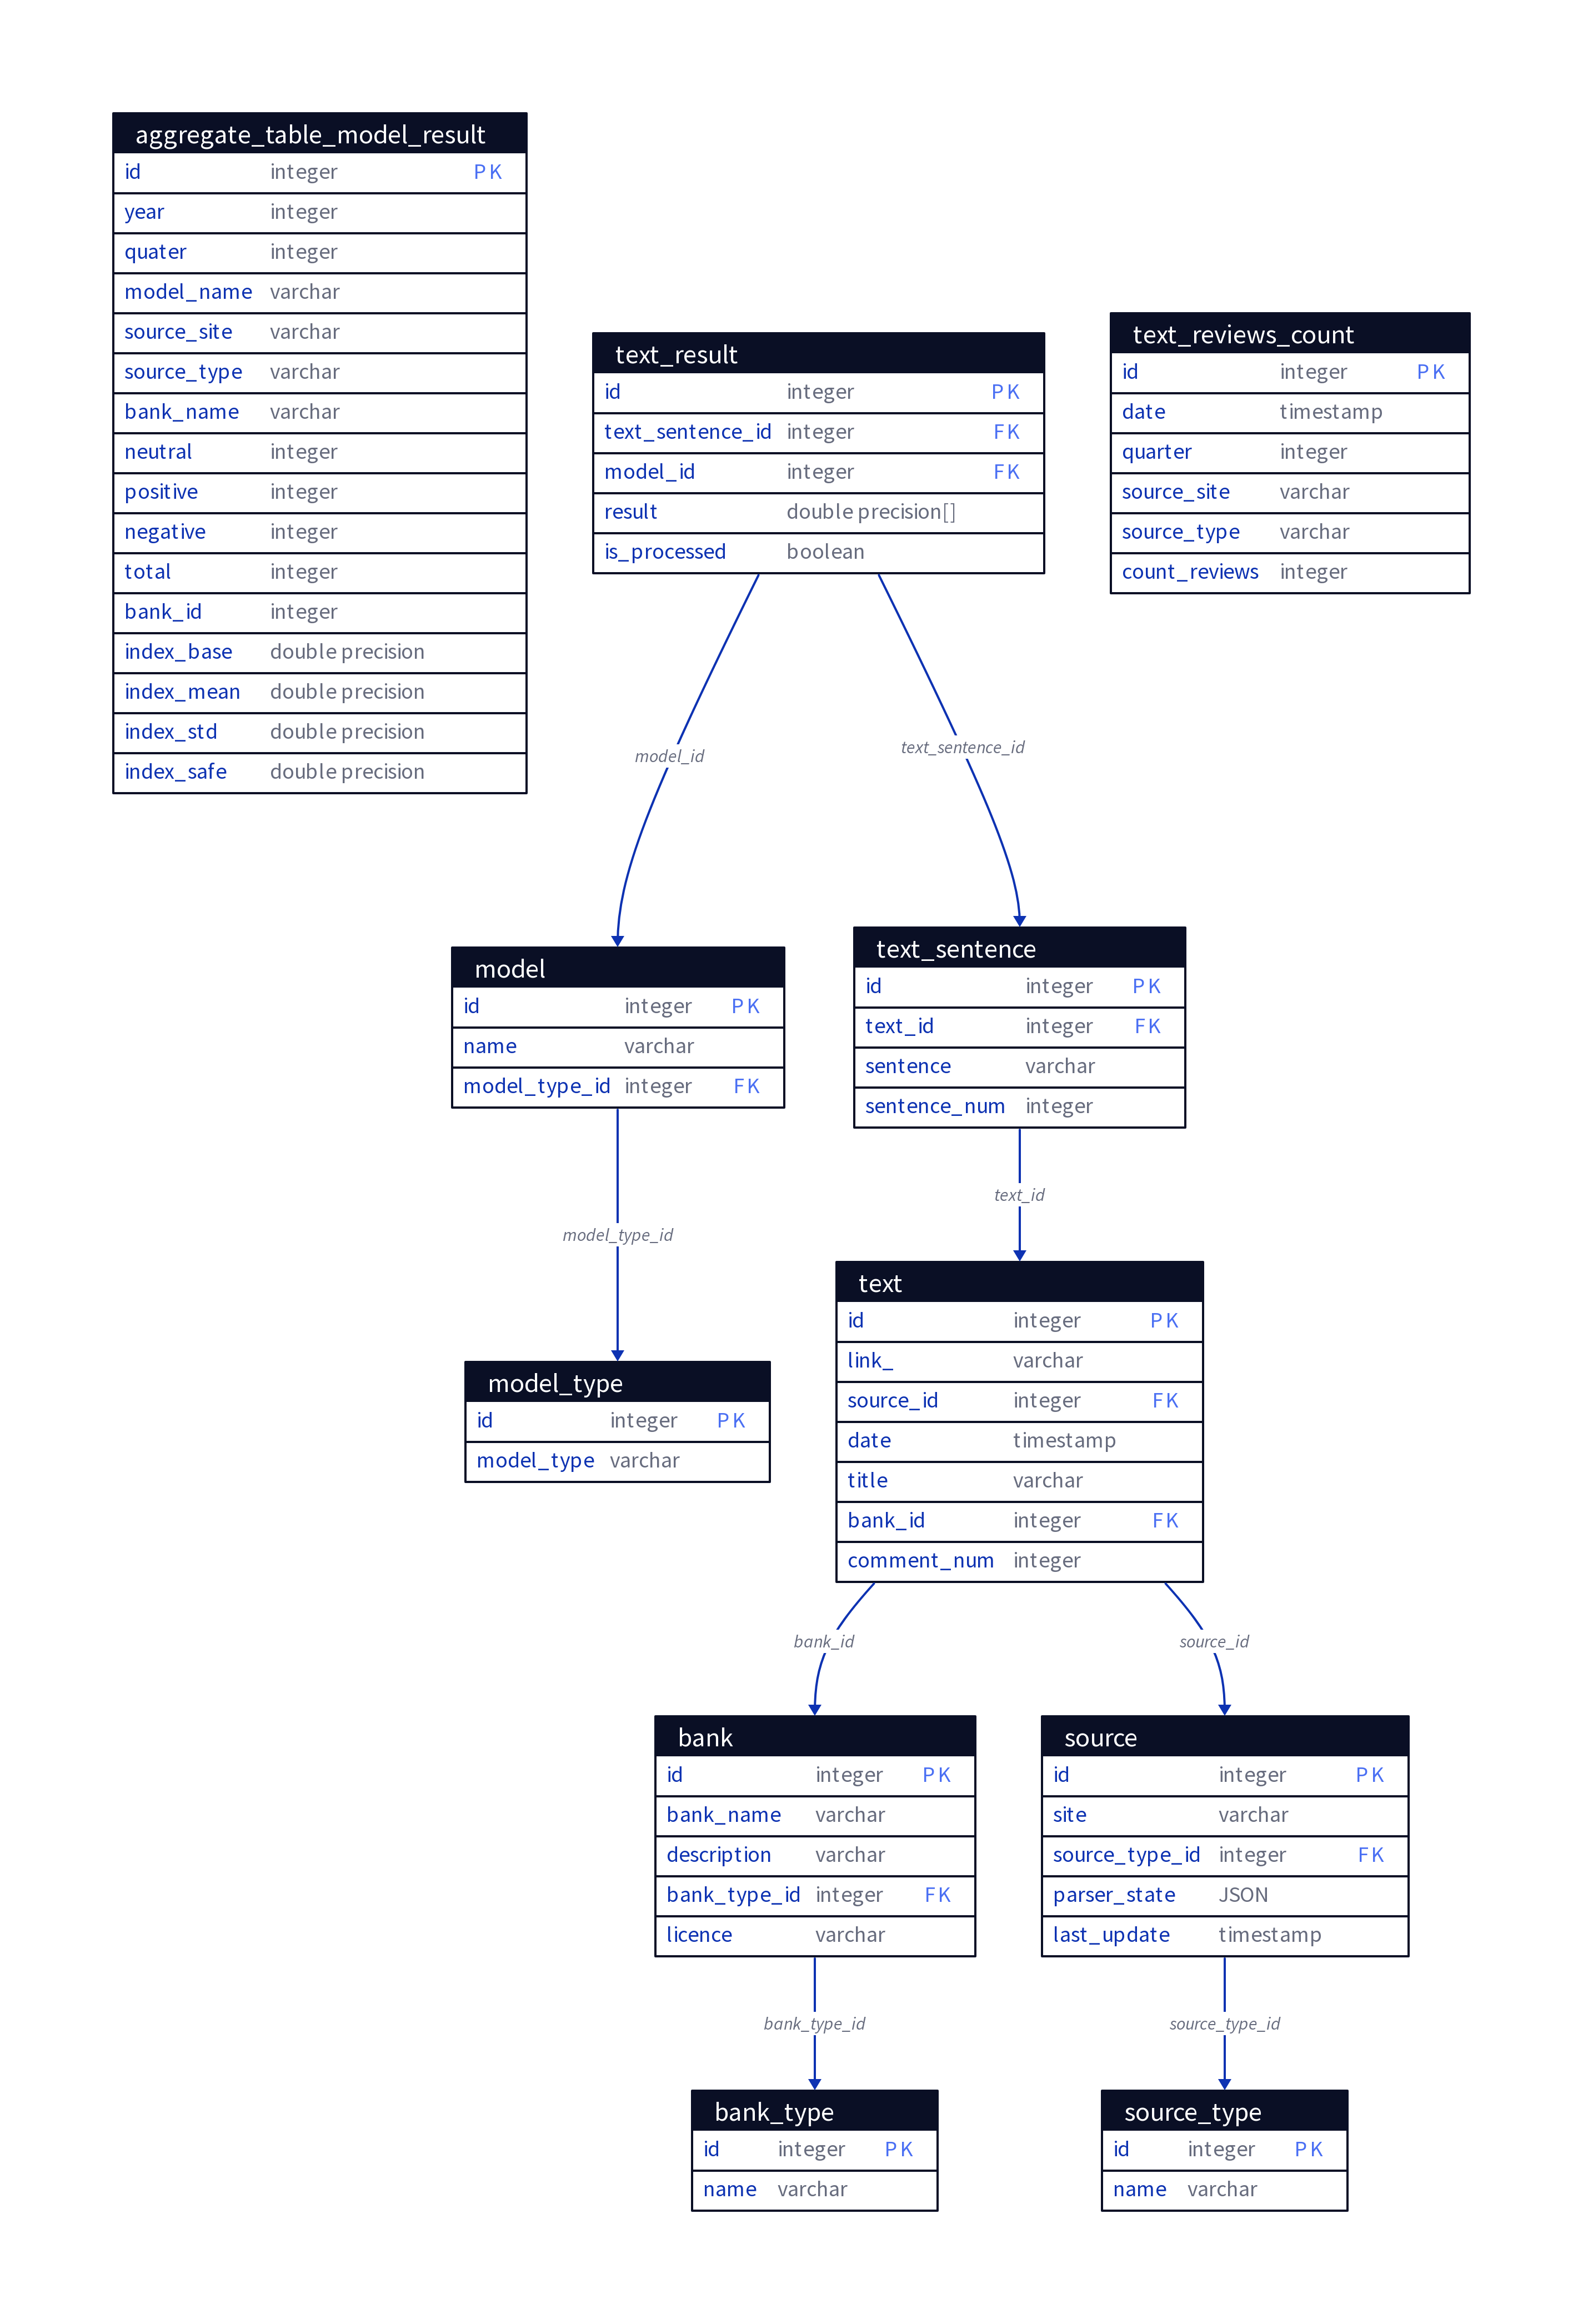
\includegraphics[width=0.8\textwidth]{img/d2/database.png}
\caption{\label{fig:database}Схема базы данных}
\end{figure}

\begin{figure}[h!]
\centering
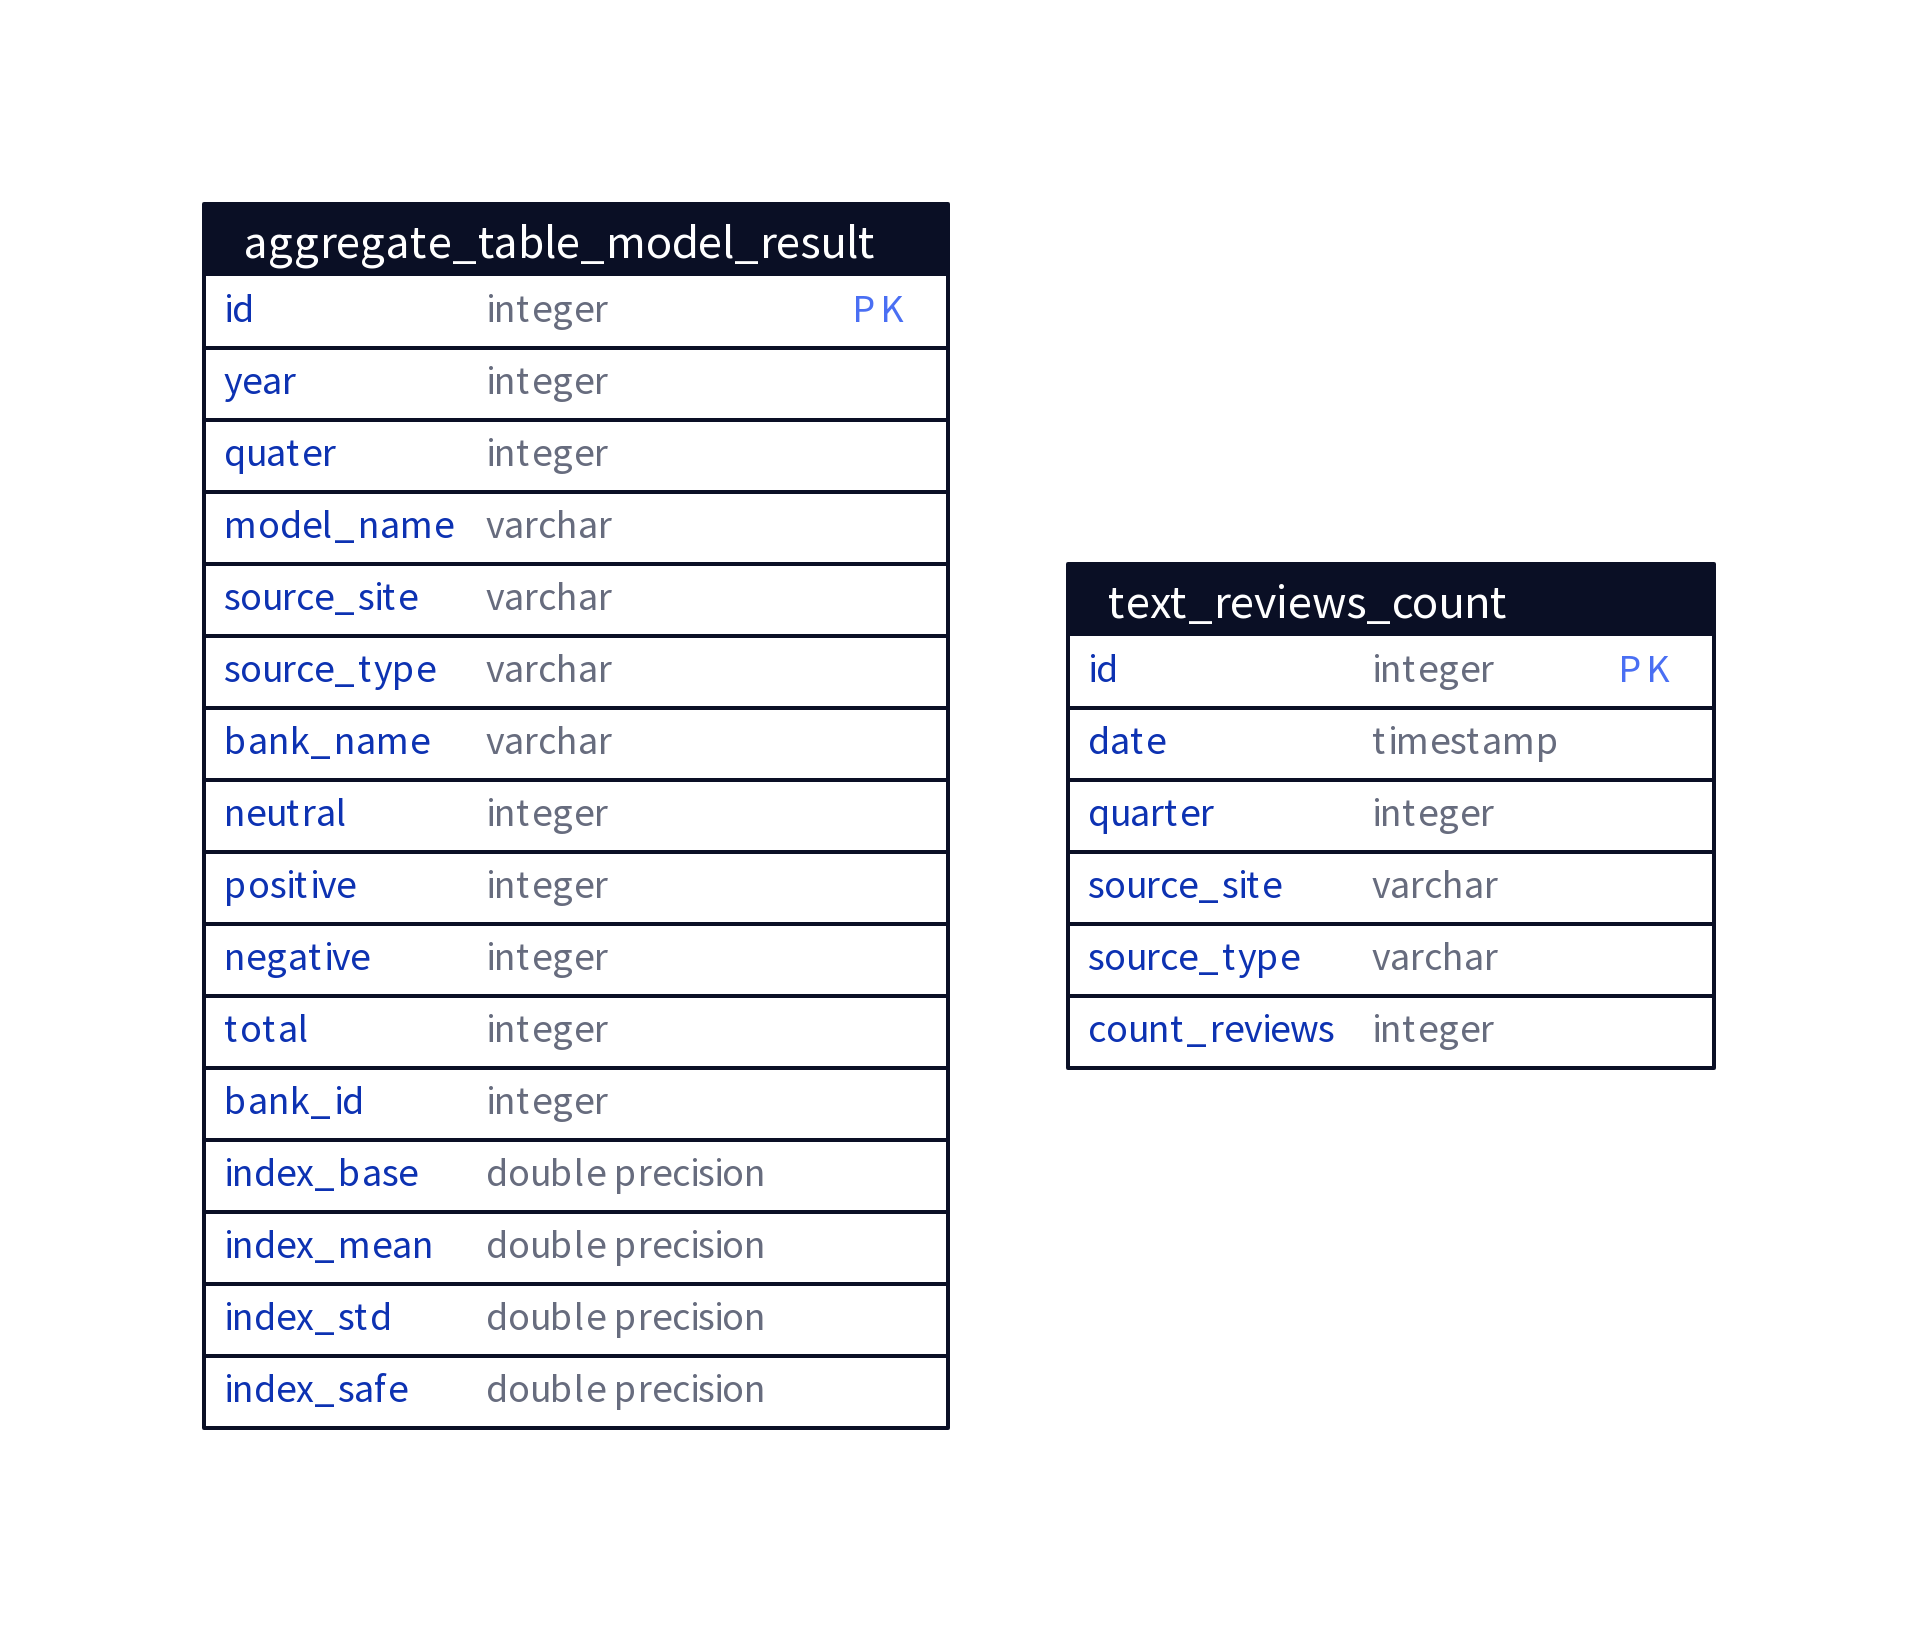
\includegraphics[width=0.8\textwidth]{img/d2/views_database.png}
\caption{\label{fig:database_views}Схема базы данных для агрегаций}
\end{figure}

\begin{figure}[h!]
\centering
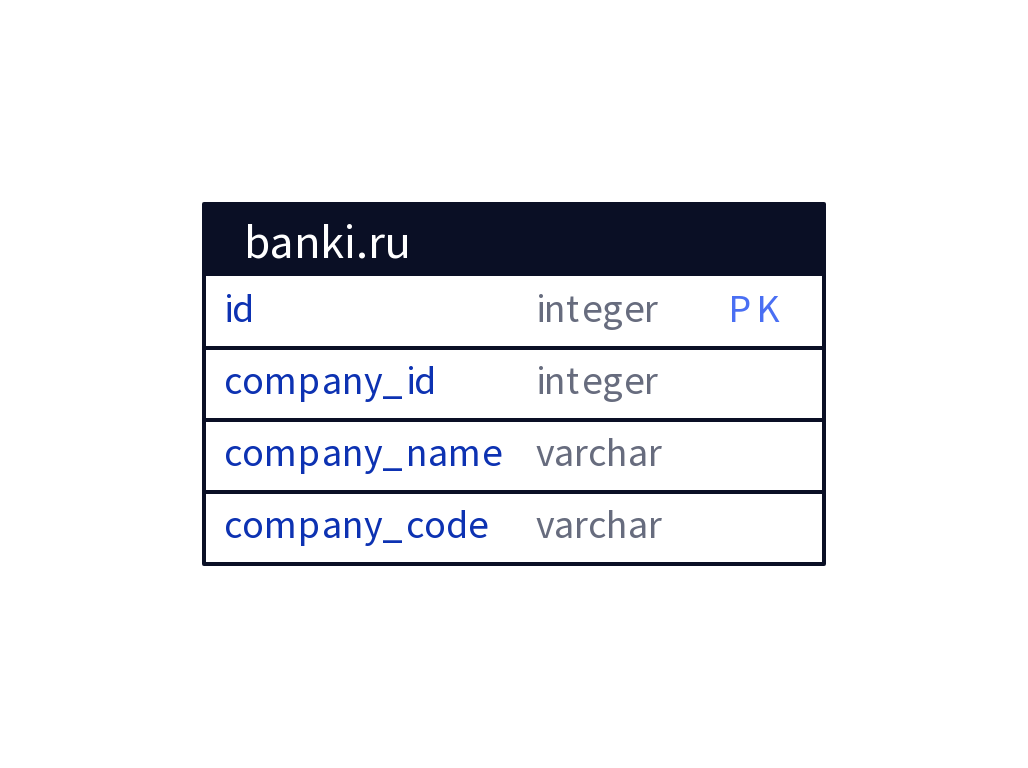
\includegraphics[width=0.8\textwidth]{img/d2/banki_ru.png}
\caption{\label{fig:database_banki_ru}Схема базы данных сайта banki.ru}
\end{figure}

\begin{figure}[h!]
\centering
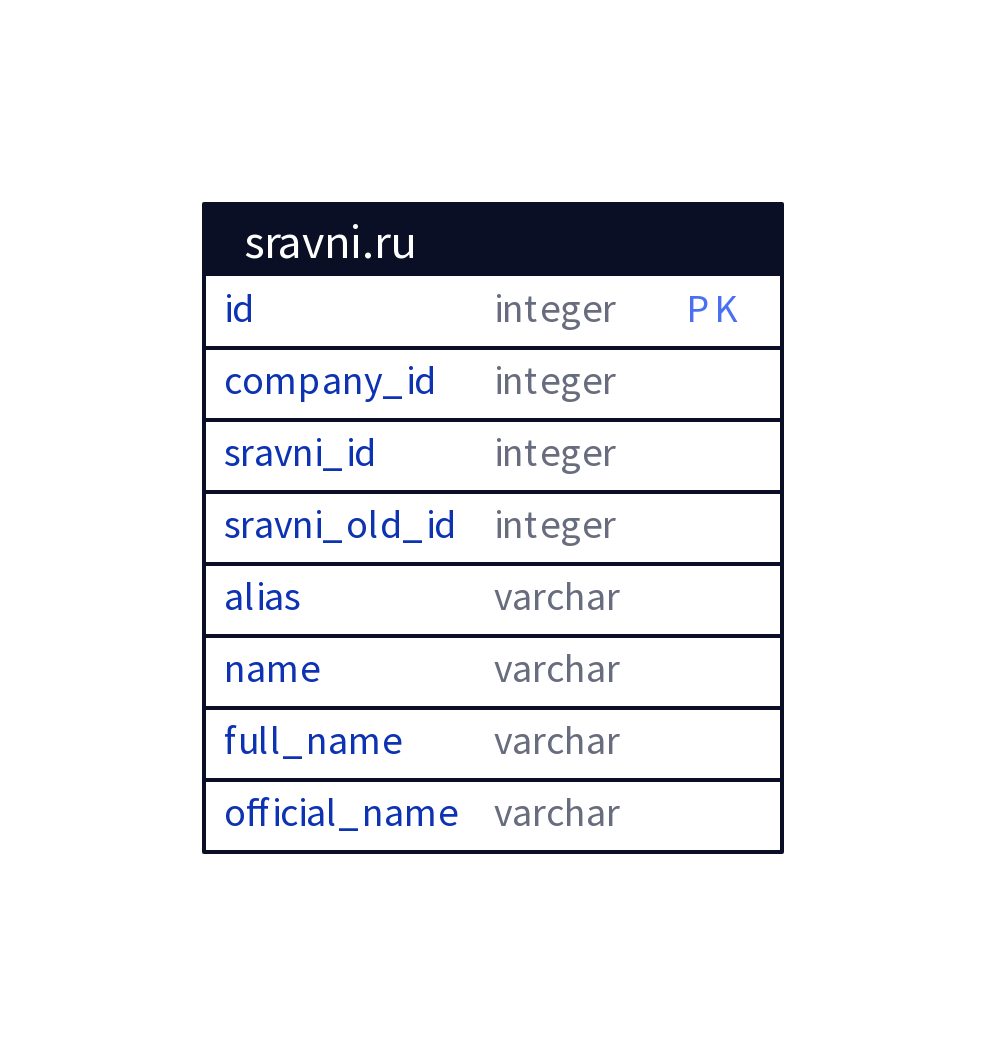
\includegraphics[width=0.8\textwidth]{img/d2/sravni_ru.png}
\caption{\label{fig:database_sravni_ru}Схема базы данных сайта sravni.ru}
\end{figure}

\begin{figure}[h!]
\centering
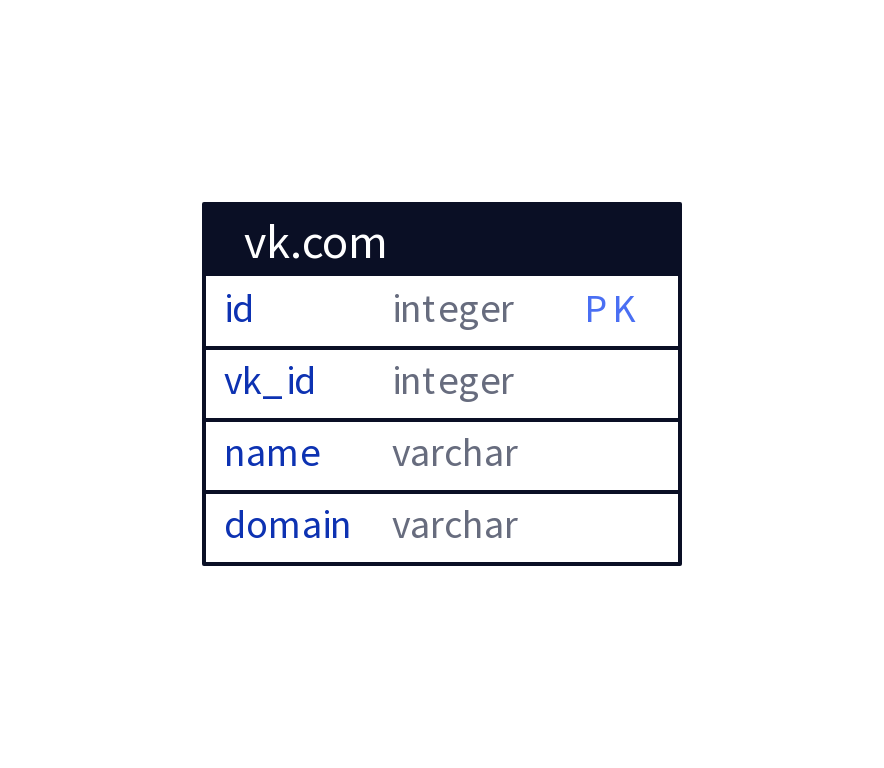
\includegraphics[width=0.8\textwidth]{img/d2/vk_com.png}
\caption{\label{fig:database_vk_com}Схема базы данных сайта vk.com}
\end{figure}
\end{document}
